\chapter{Functional modeling of idiopathic pulmonary fibrosis}\label{Yuwen_ModelBasedAnalysis}
In Chapter 4, HRCT based quantitative analysis and shape analysis methoda were developed to provide a consistent way of describing the features and progressions of IPF disease. However, it is not clear how - or whether - the spatial distribution of tissue abnormalities in IPF (including classifications of tissue type) correlate with lung function and their change over time, and currently, how to translate these imaging and shape biomarkers into functional biomarkers to directly help with the clinical diagnosis and treatment is still a challenging work. For the patient with IPF, V/Q mismatching and hypoxemia are frequent occurrences. Computational modeling provides a reliable way to simulate how these quantitative indexes contribute to the decline of lung function, therefore build a relationship between image-based biomarkers and functional presentations. This chapter outlines the functional modeling of IPF. The quantitative tissue-level and shape-level features combined with pulmonary functional test (PFT) were used to guide a patient-specific computational modeling of lung function of IPF. The lung function of old normal people was modeled as well for comparison. This work aims to integrate data from volumetric imaging, PFTs, and computational models for lung function, to understand differences between IPF and normal older lungs. The lung function of IPF has been described in Chapter 2, and the respiratory function in older people will be introduced in Section \ref{OlderRespiratory}.

%%% Section 1
\section{Respiratory function in older people} \label{OlderRespiratory}
The respiratory system of human keeps developing during the whole life, with the high-point of pulmonary function achieved before 30 years old \citep{janssens1999physiological,sprung2006age}. For most people, respiratory performance begins to gradually decline after reaching the maximal status. The ability of the lung to deliver oxygen to tissues decreases by four times from age 20 to age 70 in healthy people \citep{smith1986respiratory,zaugg2000respiratory}. Even in older athletes who experience vigorous endurance exercise and have better aerobic ability, the functional capability of lung will progressively deteriorate over time \citep{mittman1965relationship, pollock1997twenty, mcclaran1995longitudinal}. 

The aging-related changes in respiratory physiology are usually associated with structural alterations in both lungs, dilatation of alveoli, enlargement of airspaces, decrease in exchange surface area, and increased residual volume (RV) and functional residual capacity (FRC) \citep{sprung2006age,lalley2013aging}. There is a reduction in chest wall compliance and the static elastic recoil of the lung, which will lead to static air-trapping, decrease in \gls{vc}, decrease in expiratory flows and increasing work of breathing compared with younger individuals \citep{sprung2006age}. The strength of respiratory muscles decreases with age, and this is strongly correlated with nutritional status (lean body mass, body weight) and cardiac index \citep{janssens1999physiological}. The V/Q ratio heterogeneity tends to diminish results from a closing of dependent airways, and carbon monoxide transfer capability also decreases which is associated with the reduced alveolar surface. Interestingly, despite of these changes, gas exchange almost maintains normal both at rest and during exertion, with only a slight reduction in arterial oxygen tension, but no significant change in arterial carbon dioxide tension \citep{janssens1999physiological}. These age-associated changes are summarized and described in detail in Table \ref{tab:AgeingAlterations}.

\newcolumntype{C}[1]{>{\centering\arraybackslash}p{#1}}
\begin{table}[htbp]
\centering
\caption{Age-associated changes in respiratory function and their relationships to clinical presentations (Reproduced from \citep{sprung2006age, lalley2013aging})}
\label{tab:AgeingAlterations}
\begin{tabular}{p{5.8cm} p{3.6cm} p{4.8cm}}
\hline
\bf{Measurements} & \bf{Changes, $\geq$ 60 yrs.} & \bf{Clinical presentations} \\ 
\hline
\bf{Static lung volumes} &  &  \\
- TLC & Unchanged & \\
- FRC & Increase & \\
- IRV & Modest increase & \\
- ERV & Increase & \\
- TV & Modest increase & \\
- VC & Decrease & \\
- IC & Increase & \\
- RV & Increase & Impaired gas exchange\\
\hline
\bf{Dynamic lung volumes} &  &  \\
- FVC & Decrease & \\
- $FEV_1$ & Decrease & \\
- $FEV_1/FVC$ & Decrease & \\
- Peak expiratory flow & Decrease & \\
\hline
\bf{Resistance and compliance} &  &  \\
- Respiratory system resistance & Increase & \\
- Small airways closure & Increase & Impaired gas exchange\\
- Chest wall compliance & Decrease & Increase in work of breathing\\
- Lung compliance & Increase & Decrease in ventilatory response to exercise\\
\hline
\bf{Respiratory (muscle) pressures} &  &  \\
- Mean pleural pressure & Unchanged & \\
- Respiratory muscle strength & Increase & \\
\hline
\bf{Gas transfer} &  &  \\
- Ventilation-perfusion mismatch & Increase & Impaired gas exchange\\
\hline
\bf{Altered control of breathing} &  &  \\
- Responsiveness to imposed respiratory loads & Decrease & Hypoventilation\\
- Responsiveness to hypoxemia and hypercarbia & Decrease & Hypoxemia and hypercarbia\\
- Sensitivity to anesthetic agents and opioids & Increase & Respiratory failure in early postoperative period\\
\hline
\end{tabular}
\begin{tablenotes}
        \footnotesize
        \item{TLC: total lung capacity; FRC: functional residual capacity; IRV: inspiratory reserve volume; ERV: expiratory reserve volume; TV: tidal volume; VC: vital capacity; IC: inspiratory capacity; RV: Residual volume; FVC: forced vital capacity; $FEV_1$ : forced expiratory volume in 1 s; $FEV_1/FVC$ : the ratio of the forced expiratory volume in the first one second to the forced vital capacity of the lungs.}
\end{tablenotes}
\end{table}

\subsection{Aging-associated alterations in chest wall and respiratory muscle function} \label{ChestWallChange}
Several morphological changes occur in chest wall and diaphragm in older people that reduce the capability and efficiency of respiratory system. One of the most important changes is the progressive decline in chest wall compliance, which relates to the decrease of cross sectional areas of intercostal muscles, calcification of costal cartilage and rib-vertebral articulations, and narrowing of intervertebral disk spaces \citep{murray1986normal, crapo1993aging}. The structural changes in chest wall has been found to be associated with the reduction in the curvature of diaphragm and maximal transdiaphragmatic pressure, however the thickness of the diaphragm seems not change significantly with older adults \citep{zaugg2000respiratory, sprung2006age}. It is noted that the age-associated osteoporosis results in a shape change of the thorax geometry, that is an increase in dorsal kyphosis and anteroposterior chest diameter \citep{janssens1999physiological,sprung2006age}. 

The reduction in respiratory muscle strength caused by the age-related decrease of maximal static inspiratory and expiratory pressures will lead to lower efficiency of respiratory muscle activity \citep{wijesinghe2005effect,sprung2006age,lalley2013aging}. It has been proved that the reduced respiratory muscle strength is associated with the deficient nutritional status in older people, and a strong relationship was found between maximal inspiratory/expiratory pressure and lean body mass \citep{arora1982respiratory,janssens1999physiological}. Meanwhile, some study has shown that the electromyographic signal produced by twitch stimulation decreases by around 50\% in the 70-year-old people (average 73) compared with young subjects, and this reduction is attributed to the loss of type II fast-twitch muscle fibres \citep{larsson1983histochemical}. 

\subsection{Aging-associated alterations in pulmonary mechanics and lung volumes}
Although the chest wall becomes stiffer in older people, their lung parenchyma actually become more compliant \citep{mittman1965relationship, turner1968elasticity, zaugg2000respiratory}. The elastic recoil pressure of lung tissue gradually reduces by aging, with a decrease rate around 0.1 to 0.2 $cmH_2O$ on average every year \citep{turner1968elasticity}, and this reduction is attributed to the alterations in the spatial distribution of the elastic fibre network \citep{sprung2006age}. In older people, it can be observed that the static pressure-volume curve of the lung was shifted to the left, in contrast, the pressure-volume curve of the thorax was shifted to the right \citep{zaugg2000respiratory,sprung2006age}.

The tidal volume experiences a slight decrease by aging, whereas the respiratory rate gradually increases \citep{sprung2006age}. As mentioned in Section \ref{ChestWallChange}, the chest wall becomes stiffer by aging, while the lung tissues become more compliant. These changes will lead to an increase in RV and a decrease in VC \citep{lalley2013aging}. Some research indicates that RV volume will increase by approximate 50\% from 20-year-old to 70-year-old averagely, and VC will drop to around 75\% of the peak value during this period, with a decrease of 20 to 30 ml per year \citep{janssens1999physiological, sprung2006age}. The TLC, which is the the air volume in the lungs with a maximum respiratory effort, remains unchanged with age, as the effect of the decreased inward elastic recoil of the lung is offset by the reduction in the outward elastic recoil of the chest wall \citep{sprung2006age}. However, the FRC increases by 1 to 3\% per decade, since the rate of decrease in lung recoil exceeds the rate of decrease in chest wall \citep{janssens1999physiological, lalley2013aging}. Forced vital capacity (FVC) and forced expiratory volume in one second (FE$V_1$) have been demonstrated to decrease progressively with aging in both men and women \citep{knudson1976maximal}, but the volume reduces more rapidly in males than in females \citep{crapo1993aging}. FE$V_1$ decrease by 20 ml approximately per year in subjects aged 25 to 29 years, but for people more than 65 years old, the average annual rate of reduction is dramatically up to 38 ml \citep{brandstetter1983aging}.

\subsection{Aging-associated alterations in gas exchange}
The inhomogeneity of, or mismatch behavior of ventilation and perfusion increases with age, especially in gravitational dependent regions of the lung where intrapleural pressure becomes higher and the lung tissues become less elastic to keep small airways open \citep{holland1968regional, paoletti1985reference, lalley2013aging}. The increased ventilation-perfusion heterogeneity results in a reduction in $P_a O_2$, with a progressive drop from approximate 95 mmHg at 20 years to about 75 mmHg at 70 years. However, $Pa CO_2$ remains almost unchanged with increasing age, although $Pa O_2$ declines \citep{wahba1983influence, sprung2006age}. This can be probably explained by the decreased rate of basal metabolism and the higher diffusive capability of $CO_2$ across the alveolar-capillary membrane \citep{ levitzky1984effects}. Pulmonary perfusion can also reduce with age in some regions where are well ventilated but not fully perfused, and this alteration is associated with the reduced cardiac output \citep{levitzky1984effects,lalley2013aging}. The alveolar-arterial pressure difference for oxygen ($P_{A-a} O_2$) increases by aging due to the increased heterogeneity of V/Q, and is probably also related to the increase in closing volume during breathing \citep{janssens1999physiological}. It can be observed that the arterial oxygen tension reduces at a rate of approximately 5 mm Hg per decade from the age of 20 years, and the increasing alveolar-arterial oxygen gradient and the decreased arterial oxygen tension are expected to be the main reason of the impaired arterial oxygenation in elder people \citep{smith1986respiratory,zaugg2000respiratory}. Additionally, the diffusing capacity of the lungs for carbon monoxide (DLCO) decreases with aging \citep{guenard1996pulmonary}, with about 0.3 $mL.min^{-1}mmHg^{-1}$ and 0.2 $mL.min^{-1}mmHg^{-1}$ for men and women, respectively \citep{murray1986normal}. The reduction is more significant after 40 yrs of age, and the increased mismatch in V/Q, a decline in the alveolar surface area \citep{verbeken1992senile, thurlbeck1975growth}, the decreased density of lung capillaries \citep{butler1970capillary} and the reduction in pulmonary capillary blood volume \citep{guenard1996pulmonary} are all potential factors to cause the impaired diffusion capacity.

\section{Methods: Patient-specific modeling of IPF lung function}
In this section, a patient-specific computational model of lung function is proposed to explore the V/Q matching and the whole lung gas exchange for patient with IPF. In order to make a comparison of lung function between IPF patient and older normal people, for each patient, a subject-specific lung mesh that represents the statistical lung shape of old normal individual with the same age, BMI and pulmonary functional data was predicted using SSM. Anatomically based airway and blood vessel trees were generated derived from HRCT images, respectively matched to IPF lung mesh and the corresponding old normal lung mesh. The ventilation, perfusion and gas exchange models were then constricted to simulate $\dot{V}$, $\dot{Q}$ distribution and gas transport in normal and disease constricted condition, respectively. During this process, individual's lung parenchymal tissue classification and quantification data was mapped to model of IPF patient, with fibrosis reducing tissue compliance and narrowing vessels. Data from PFTs were used to parameterize the models and set the boundary conditions. The framework of modeling is illustrated in Figure \ref{fig:WholeFramework}. 

\begin{figure*}[htbp]
  \centering 
  
\includegraphics[height=6.2in]{ModelBasedAnalysis/Image/WholeFramework.png}
  \caption{Computational modeling framework for IPF and older normal lung function. }
  \label{fig:WholeFramework}
\end{figure*}

\subsection{Clinical data}
Two patients diagnosed with IPF were selected from the clinical data used in Chapter 4 as representative subjects for functional modeling. Patient 1 is female which has three time points with 12 and 23 month interval, respectively, and patient 2 is a male which has two time points with 46 month interval. The clinical data for each patient includes both HRCT images and PFT results, with less than 3 months between the scan date and the PFT date. 

\subsection{Construction of lung lobe geometry}
In Chapter 4, Section \ref{VolumeAnalysis} and \ref{SSMBasedAnalysis}, we compared the lung lobe shapes and volumes of IPF patients with old normal people. It can be observed that there is a significant difference of lung lobe geometry between IPF and old normal groups, and this alteration in lung shape mainly focuses on the basal part (lower lobe), strongly associated with the distribution of fibrosis in IPF. In order to involve the impact of shape change into the modeling of lung function, SSM of old normal people and patient's individual information were combined to predict an average lung lobe shape of old normal as a control group for each IPF patient. Meanwhile, the lung lobe mesh of each IPF patient was generated using the method introduced in Chapter 3, Section \ref{ShapeModelGeneration}.

\subsubsection{Relationship between lung function and lung shape}
It is supported by evidence that the age-related changes in lung structures are strongly associated with a series of alterations in respiratory functions (introduced in Section \ref{AgingRespiratory}). For example, the reduction in chest wall compliance of old people leads to a decrease in VC, while an increased RV in elders usually results in impaired capability of gas exchange which relates to a lower measured DLCO. In a previous study from our research group, the lung structure-function relationships were analyzed through quantifying the correlations of the first three PCA-based mode weights calculated from old normal SSM (introduced in Chapter 3, Section \ref{MeshPrediction}, and Chapter 4, Section \ref{SSMBasedAnalysis}) with age, BMI, lung volume and some pulmonary function measurements. For each training subject of SSM, the individual weight scores for each of the first three shape modes which captures most shape variation were examined. An ordinary least squares regression was applied to test the associations, and P value was used to quantify the strength of each association, with an alpha level of 0.05 considered statistically significant. Analysis result illustrates that Mode 1 has positive relationship with $FEV_1$, $FEV_1/FVC$, Maximal mid-expiratory Flow (FEF25\%-75\%), BMI and DLCO, while has negative correlation with age, RV and RV/TLC. For Mode 2, only BMI is found a correlation with the shape variation, whereas quite a number of lung volume measurements, including FRC, TLC ,VC and RV show strong relationship with scores of Mode 3.

\subsubsection{Shape prediction of old normal lungs}
The lung shape prediction of old normal people was developed based on the previous analysis of lung structure-function relationship. Age, BMI, FVC, $FEV_1$, FRC, TLC, VC, RV, RV/TLC and DLCO were selected as the individual functional measurements to train the lung shape predictive model, as these parameters show relatively strong correlations with the first three shape modes. The training process of lung shape predictive model is to find optimized equations that can best describe the relationship between the functional measures and the mode weights. For each shape mode, a multivariate regression model was constructed as follows:

\begin{equation}
 \label{eq:MultivariateRegression}
 w_i = \alpha_{0i} + \alpha_{1i}m_1 + \alpha_{2i}m_2 + ... + \alpha_{ni}m_i + \varepsilon,
\end{equation}

\noindent where $w_i$ is the weight score of the ith shape mode, n is the number of functional measures, $\alpha_{0i}, \alpha_{1i} ... \alpha_{ni}$ are the regression coefficients, in which $\alpha_{0i}$ is the intercept, $m_i$ is the tested value of the ith functional measure, $\varepsilon$ is a random error. Here, it is assumed that all the functional measures are independent variables.

Using Equation \ref{eq:MultivariateRegression}, a set of possible regression models can be developed for each shape mode (with different regression coefficients $\alpha_{0i}, \alpha_{1i} ... \alpha_{ni}$). In order to find the best predictive model from all the possible models, two most common criterions for model selection, \gls{aic} and \gls{bic}, were used to deal with the trade-off between the goodness of fit of the model and the simplicity of the model. Both AIC and BIC are founded on information theory, with calculated by:

\begin{equation}
 \label{eq:AIC}
 AIC = 2k - 2lnL(\theta),
\end{equation}

\begin{equation}
 \label{eq:BIC}
 BIC = ln(n)k - 2lnL(\theta),
\end{equation}

\noindent where k is the number of the estimated parameters (that is functional measures in this study) in the model, $L(\theta)$ is the maximized value of the likelihood function of the model and $\theta$ are the parameter values that maximize the likelihood function.

The multivariate regression models with the lowest value of AIC and BIC were selected as the best predictive models, then the models of the first three PCA modes were constructed in the form of Equation \ref{eq:MultivariateRegression}, shown as follows:

\begin{equation} 
 \label{eq:TerminalBoundaryCondition}
 \begin{split}
 & w_1 = 1.38 + (-0.04 \times Age) + (0.38 \times FVC) + (-0.04 \times DLCO), \\
 & w_2 = 3.49 + (-0.16 \times BMI) + 0.02 \times RV/TLC, \\
 & w_3 = 4.90 + (-0.02 \times Age) + (-0.45 \times TLC) + (-0.05 \times DLCO), \\
 \end{split}
\end{equation}
 
\noindent where $w_1$, $w_2$ and $w_3$ are the weight scores of the first three shape modes. Through inputting the individual functional measures into the regression models, the weights of first three modes can be calculated. Then the subject-specific predicted shape of old normal lung can be reconstructed with adding linear combination of the first three modes into the average SSM:

\begin{equation}
 \label{eq:NormalLungPrediction}
 S_{pred} = S_{mean} + \sum_{i=1}^3 \mathbf{u}_i w_{i},
\end{equation}

\noindent where $S_{mean}$ is the mean shape of SSM for older normal people, $S_{pred}$ is the subject-specific predicted lung shape. 

\subsection{Construction of airway/vasculature geometry} \label{AirwayVesselGeometry}
Subject-specific conducting airway trees and pulmonary vasculature trees were constructed in both IPF and predicted old normal lung mesh. The  geometry of pulmonary airway and vasculature are representative of the important structural features of the pulmonary circulation, therefore are the basis on which the following anatomically based functional models can develop. In this section, airway/vasculature trees were firstly generated with filling 1-D finite element branches in the predicted old normal lung mesh, then were deformed to the shape of IPF lung mesh which presents a compression effect in the lower lobes in our previous analysis. The airway/vasculature diameters were assigned to each branch as a postprocessing step specific to IPF and old normal geometry respectively. Using this way, the branches of IPF and old normal airway/vasculature will be kept in the same geometric connectivity and same lobar distribution, but with different radius and length. 

\subsubsection{Airway tree}
In order to generate airway tree in the lung shape, the bi-cubic Hermite finite element mesh of lung surface was converted to a tri-cubic Hermite volumetric mesh which has been introduced in Chapter 4, Section \ref{DataNormalization}. An anatomical based structure of the bronchial airways (from trachea to terminal bronchioles) was generated using the methods developed by Tawhai et al, as described in details in \cite{tawhai2000generation, tawhai2004ct}. In brief, the centerlines of the largest airways (trachea, left and right pulmonary airway branches of the first 6 generations) were manually segmented from the subject's HRCT images, which provides an incomplete description of the airway tree. Then, the larger airways was used as initial condition to generate the branches down to the level of the terminal bronchioles (smaller airways) within the subject's lung mesh using a volume-filling branching algorithm. The steps to generate patient-specific airways in IPF and old normal lungs were summarized as follows:

1. 1-D finite element mesh of the centerlines of IPF larger airways were created manually from HRCT raw images of IPF patient (shown in Figure \ref{fig:AirwayGeneration-a}).

2. The 1-D tree of central airways obtained above was mapped to the volumetric mesh of old normal lung. The nodal positions inside the mesh were mapped through calculating the local coordination $\xi_{i}$ with respect to its element (details in Chapter 4, Section \ref{DataNormalization}). The branches outside the mesh were then scaled to match the target lung volume, followed by a manual adjustment. The element connectivity remains the same during mapping.

3. The mapped larger airway in step 2 was used as a starting geometry for generating a full airway tree by volume-filling branching algorithm \citep{tawhai2000generation, tawhai2004ct}, to fill the lung-shaped of old normal volumetric mesh. Briefly, uniformed spaced grid seed points were created within the 3D volumetric lung mesh. The number of seed points is around 32000 (45\% for left lung and \%55 for right lung) which equals to the number of pulmonary density of acinar units in the lung \citep{haefeli1988morphometry}. The branching algorithm was designed to generate a branching structure recursively towards the center of mass of seed point units, until each seed point was assigned a terminal bronchiole (shown in Figure \ref{fig:AirwayGeneration-b}). 

4. The generated linear mesh of full airway tree in step 3 was mapped back to the volumetric lung mesh of IPF patient using the same method in step 2.

\begin{figure}[htbp] 
\centering
\begin{subfigure}{.53\linewidth}% set image scale
  \sbox0{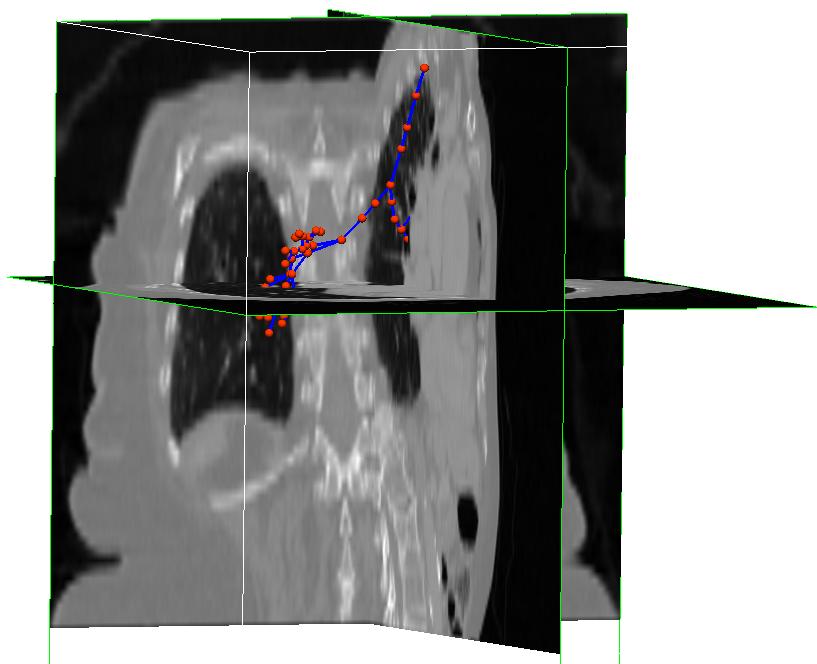
\includegraphics{ModelBasedAnalysis/Image/IPF511_UpperAirwayDigitizing3.png}}
  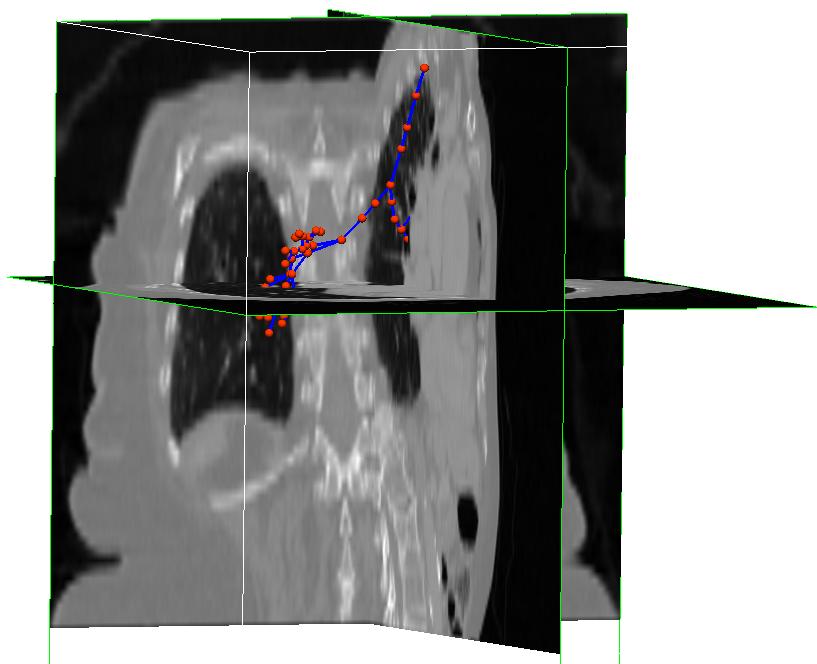
\includegraphics[width=\linewidth,trim={{.0\wd0} {.0\wd0} {.0\wd0} {.0\wd0}},clip]{ModelBasedAnalysis/Image/IPF511_UpperAirwayDigitizing3.png}
  \caption{Manual digitized upper airway}
  \label{fig:AirwayGeneration-a} 
\end{subfigure}
%\vspace{.1in} % control space between the upper context and figure
\hspace{.1in} % control space between two figures
\begin{subfigure}{.425\linewidth}% set image scale
  \sbox0{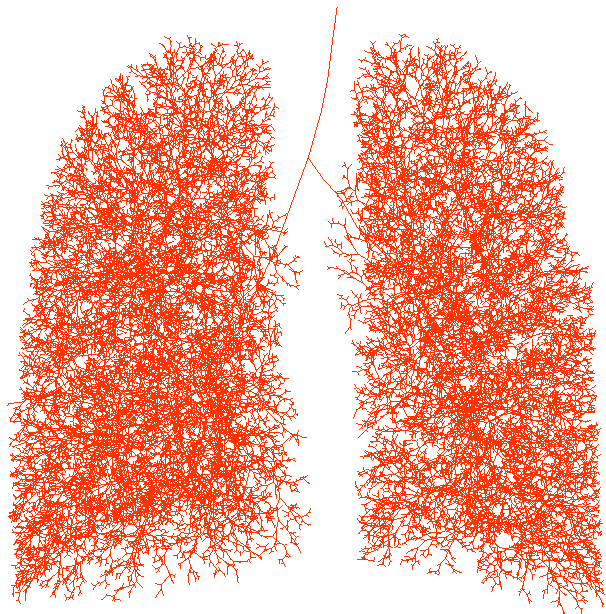
\includegraphics{ModelBasedAnalysis/Image/IPF511_Normal_FE_Airway.png}}
  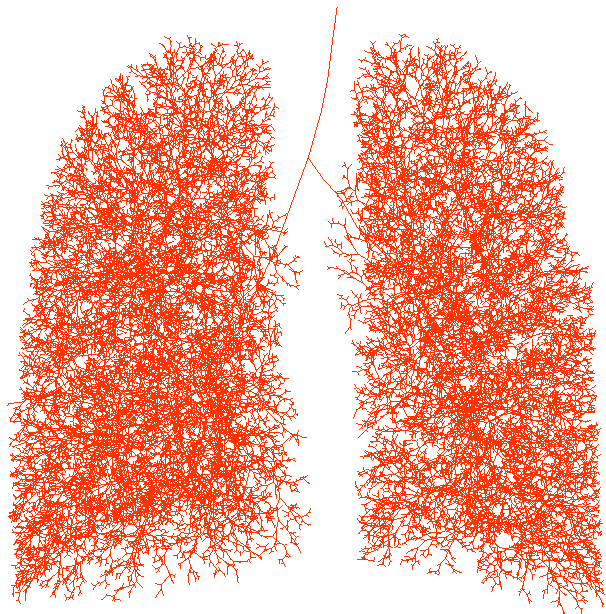
\includegraphics[width=\linewidth,trim={{.0\wd0} {.0\wd0} {.0\wd0} {.0\wd0}},clip]{ModelBasedAnalysis/Image/IPF511_Normal_FE_Airway.png}
  \caption{Full airway tree}
  \label{fig:AirwayGeneration-b} 
\end{subfigure}
\caption{Generation of airway tree. (a) Manual digitized upper airway tree from HRCT images in 3D. Blue lines are the centerlines of upper airway tree, and red points represent airway nodes. (b) Geometry of full conducting airway tree generated using volume-filling algorithm. The
model is shown from the anterior view, with the left lung on right, and right lung on left.} 
\label{fig:AirwayGeneration}
\end{figure}

In the next stage, the diameters of airway branches were calculated for both IPF and old normal geometry, the method proceeds as follows:

1. The trachea radius of IPF was measured from segmented HRCT images through averaging the values at the position of 1/4, 1/2 and 3/4 along the centerline of the trachea, with treating trachea as a circular cross-section.

2. Radius of the terminal branch of IPF was assumed to be constricted based on a found that 70\% of the IPF patients occur narrowed airways \citep{crystal1976idiopathic}. The radius of narrowed terminal branch was calculated by:

\begin{equation}
 \label{eq:NarrowedTerminalRadius}
 RdT_{IPF} = RdT_{normal} \times \sqrt[3]{\frac{FRC_{IPF}}{FRC_{Normal}}},
\end{equation}

\noindent where $FRC_{IPF}$ is the measured FRC volume of IPF patient and $FRC_{Normal}$ is the reference FRC volume of old normal people obtained from PFT report. $RdT_{normal}$ is the terminal bronchiole radius of normal lung, estimated to be around 0.2mm \citep{horsfield1976diameter}. $RdT_{IPF}$ is the constricted IPF terminal radius. 

3. Radius of the other airway branches of IPF were calculated after initializing the trachea radius and Horsfield diameter ratios ($R_dH$). The $R_dH$ was adjusted during each calculation until the terminal radius $RdT_{IPF}$ can touch the value obtained from step 3. The conducting airway volume of IPF was then acquired by summing up the branch volume from distal to the trachea.

4. It has been proved by evidence that an increase in airway volume occurs in IPF lung, therefore, here the conducting airway volume of old normal lung was predicted using a statistically measured ratio $R_{volume}$, which represents the ratio of IPF conducting airway volume to the old normal conducting airway volume \citep{plantier2016increased}. By setting up the normal terminal radius with 0.2mm and the predicted conducting airway volume, the $R_dH$ and the radius of other branches for old normal airway tree can be specially calculated. During this process, the normal range of trachea radius of the human lung (5mm to 11mm for women, 6.5mm to 12mm for man) was also taken into consideration \citep{breatnach1984dimensions} by adjusting the volume ratio $R_{volume}$ until the predicted trachea radius can reach the normal range. $R_{volume}$ was initialized as 34.2/45.3 (normal/IPF) which is the average volume ratio measured among a number of IPF patients and normal people. 

Using the above steps, patient-specific pulmonary airway geometry for IPF and old normal lung were constructed. 

\subsubsection{Vasculature tree}
The centrelines of large vessel tree (the first two generations) were manually recognized from HRCT images, represented as 1-D finite element mesh. In this thesis, the pulmonary arterial and venous trees of other generations were assumed to be approximate replicas of the airway tree. Using the airway tree to construct vessel geometry is a reasonable assumption at this level, as the pulmonary arteries generate closely surrounding the airways trees, the airways and blood vessels have similar lengths and orientations, airway and vsculature bifurcate in union from larger branch to bronchiole level, and the veins divide at the midpoint between adjacent airway bifurcations \citep{weibel1984pathway, hsia2016lung}. The manual branch of the main vessel plus the finite element of airway tree provided a full pulmonary blood vessel geometry of IPF patient. The vasculature structure of old normal was obtained using the same mapping procedure used for airway which has been described previously. Based on the vasculature model developed by Clark et al \citep{clark2010contribution,clark2011interdependent}, intra-acinar arterioles and venules (microcirvulatory system) were assumed to be connected at each generation through a ''ladder-like'' pattern that a capillary bed covers the alveoli at the acinar circulatory ''unit''.

The unstrained (zero transmural pressure ($P_{tm}$)) radius of main pulmonary artery and vein were assigned based on the patient-specific trachea radius and the data from morphometric studies \citep{horsfield1978morphometry,horsfield1981morphometry,huang1996morphometry}. The radius of all the other arteries and veins down to the distal level were calculated based on a defined rate of increase in diameter with vessel order, Strahler diameter ratio ($R_dS$). The value of $R_dS$ for arterial tree and venous tree were specified according to the radius of main artery and vein, and the consistency compared with the values from raw human data \citep{horsfield1978morphometry,horsfield1981morphometry,huang1996morphometry}. The vessel radius for IPF and old normal lung were then calculated, respectively. 
 
\subsection{Construction of computational models} \label{ComputationalModelConstruction}
In this thesis, the computational modeling of lung function integrates previously published models of ventilation \citep{swan2012computational}, perfusion \citep{clark2010contribution, clark2011interdependent} and gas exchange \citep{swan2010evidence} to simulate $\dot{V}$, $\dot{Q}$ distribution and oxygen and carbon dioxide exchange during tidal breathing in the upright posture. The patient-specific geometry of airways and vessels were used as input for these models. A brief introduction of the model components is summarized below, details can be found in the reference papers.

\subsubsection{Ventilation model}
The ventilation model developed by \cite{swan2012computational} was used to predict the time-averaged topological distribution of inhaled air in the upright human lung, governed by local tissue deformation, elastic recoil pressure, airway resistance and acinar compliance. Approximate 32000 acinar units were generated subtending each terminal bronchiole, and worked as an individual compliant compartment. The acinar volume and compliance were initialized at FRC state using the tissue mechanics model developed by \cite{tawhai2009supine}. The anatomical geometry of airways were embedded in the model, and its relationship to air flow resistance was included in the model construction. The movement of air into each acinar unit was determined by expansion of the alveolar tissue and airway resistance through a temporally changing pleural pressure.

In this model, the flow through conducting airways was assumed to be Poiseuille flow, which was fully developed and laminar with a correction factor to account for additional energy losses occurred according to the work of \cite{pedley1970energy}. Additional energy losses caused by flow disturbances were created at the airway bifurcations and involved in the calculation of pressure drop across the junction. A correction term, $Z_{Pe}$, was used to define the ratio of actual energy dissipation to Poiseuille flow dissipation, then the ratio of actural airway resistance ($R_{aw}$) to its Poiseuille flow equivalent ($R_P$) can be calculated by (ignoring kinetic energy changes):

\begin{equation}
 \label{eq:EnergyDissipation}
 Z_{Pe} = \frac{R_{aw}}{R_P} = \frac{K_{Pe}}{4\sqrt{2}}(R_e \times \frac{2r}{l})^{0.5},
\end{equation}

\noindent where $R_e$ is the Reynolds number, r and l are the radius and length of the airway, respectively. $R_e = \frac{2Q\rho}{\pi r \mu}$, where $\rho$ and $\mu$ are the density ($1.51 \times 10^{-6}g.mm^{-3}$) and viscosity ($1.92 \times 10^{-5}P_{a}.s$) of air, respectively. $K_{Pe}$ is a constant, set to 1.85. Then, the resistance of each airway branch was calculated as the Poiseuile resistance ($R_{aw}$) multiplied by the term $Z_{Pe}$, and the Poiseuille flow through conducting airway can be acquired by the following equation:

\begin{equation}
 \label{eq:PressureFlowEquation}
 P_{aw_2} - P_{aw_1} = R_{aw}R_P = Z_{Pe}R_PQ = Z_{Pe}\frac{8l\mu}{\pi r^{4}}Q,
\end{equation}

\noindent where $P_{aw_1}$, $P_{aw_2}$ are the air pressures at the start and end of airway branch, Q is the air flow through the airway. The air flow into the acinar unit (modeled as a compliant unit subtending terminal bronchiole) was derived by an equation of motion that relates airway resistance, air flow, tissue compliance and the rate of change of internal and external pressures:

\begin{equation}
 \label{eq:AcinarFlowEquation}
 P_{aw} = \frac{V_A}{C_A} + R_{aw}Q + I\frac{dQ}{dt} - P_l,
\end{equation}

\noindent where $P_{aw}$, $R_{aw}$ and Q are the pressure, Poiseuille resistance and flow in the terminal bronchiole, $V_A$ and $C_A$ are the volume and compliance of the acinar unit, I is inertance of the unit,and $P_l$ is the local pleural pressure (varied sinusoidally) working to expand the unit and drive air flow through conducting airway to terminal acinus.

Here, we assumed that the rate of change of airflow Q is small enough, therefore the item $I\frac{dQ}{dt}$ in Equation \ref{eq:AcinarFlowEquation} can be neglected. A suitable small time interval, $\Delta t = t_n - t_{n-1}$, was defined, and the flow at the end of the time period $Q_n = Q(t_n)$ (Q respect to t) can be calculated as:

\begin{equation}
 \label{eq:FlowRespectToTime}
 Q_n = C_A(\nu - \beta) + Q_{n-1} - C_A(\nu - \beta)exp(\frac{-\Delta t}{R_{aw}C_A}),
\end{equation}

\noindent where $Q_{n-1} = Q(t_{n-1})$ is the flow at the end of the previous time period. $\nu = dP_{aw}/DT$, $\beta = d_{Pl}/dt$ are the change of broncohiole pressure and pleural pressure with respect t. This equation is derived from Equation \ref{eq:AcinarFlowEquation}, the detailed description can be found in \cite{swan2012computational}.

\subsubsection{Perfusion model}
The multi-scale pulmonary perfusion model developed by \cite{clark2011interdependent} was used to simulate a time-averaged distribution of blood flow, capillary blood volume and average \gls{rbc} transit time for each acinar unit. The full vasculature structure (including arteries, veins, intra-acinar arterioles and venules, capillaries) generated in Section \ref{AirwayVesselGeometry} was embedded in this model. Distension of blood vessels and hydrostatic effects were also involved in the model, with arterial and venous diameter and the thickness of the capillary sheet assumed proportional to the transmural pressure ($P_{tm}$). The intra-acinar (extra-capillary) blood flow was modeled in a symmetric ladder structure which relates the vessel diameter, length and the thickness of capillary sheet.

Similarly to air flow, the flow through pulmonary arteries and veins was predicted using a Poiseuille equation  with a term of gravitational effects acting on the vessels, and can be described by:

\begin{equation}
 \label{eq:VesselFlow}
 \Delta P = P_{b2} - P_{b1} = \frac{128 \mu_bL\dot{Q}}{\pi D^{4}} + \rho_b Lgcos\theta,
\end{equation}

\noindent where $P_{b1}$ and $P_{b2}$ are the blood pressures at the beginning and end of the vessel element, $\mu_b$ and $\rho_b$ are the viscosity and density of the blood in the vessel, L and D are the vessel length and radius, $\dot{Q}$ is the volumetric flow rate in the vessel, g is the gravitational acceleration ($9.81m/s^2$), and $\theta$ is the angle between the vessel and the direction of gravity. 

The term $\rho_b Lgcos\theta$ in Equation \ref{eq:VesselFlow} represents the gravity effects acting on the vessels. In this model, an arteriole and an venule were joined at each generation by a capillary bed, forming a ''ladder-like'' structure, to construct the the intra-acinar circulation. Therefore, the item $\rho_b Lgcos\theta$ can be negligible if the length of acinar arterioles and venules was assumed to be small enough:

\begin{equation}
 \label{eq:VesselFlow1}
 \Delta P = \frac{128 \mu_bL\dot{Q}}{\pi D^{4}},
\end{equation}

The deformation of vessels in the axial and radial directions due to the surrounding lung parenchyma and the tethering force of lung tissues was included in the model through calculating the axial stretch from tissue deformation. The strained diameter D in Equation \ref{eq:VesselFlow1} was assumed a linear relationship with the transmural pressure $P_{tm}$ as:

\begin{equation}
 \label{eq:VesselDeformation}
 \frac{D}{D_0} = \alpha P_{tm} + 1,
\end{equation}

\noindent where $D_0$ is the unstrained vessel diameter, $\alpha$ is the vessel compliance constant. The tethering pressure acting on the blood vessel in the radial direction was assumed to be equal and opposite to the local tissue elastic recoil pressure ($P_e$), therefore $P_{tm} \approx P_b - P_e$, where $P_b$ is the average blood pressure across the vessel. Then, the blood flow through a capillary sheet ($\dot{Q}$) was modelled using the classic sheet flow theory developed by \cite{fung1969theory}:

\begin{equation}
 \label{eq:CapillarySheetFlow}
 \dot{Q} = \frac{SA}{\mu_c f l^{2}_{C}} \int\ H^{3}dP_{tm},
\end{equation}

\noindent where A is the alveolar surface area, S is the proportion of alveolar surface area (A) composed of capillaries, $\mu_c$ is the apparent viscosity of blood in the capillaries, f is the numerical friction factor, $l_C$ is the average path length through the capillary network between arteriole and venule. H is the thickness of the capillary sheet which was assumed to be approximately linearly dependent on $P_{tm}$ similar to Equation \ref{eq:VesselDeformation}:

\begin{equation}
 \label{eq:CapillarySheetDeformation}
 \frac{H}{H_0} = \alpha_C P_{tm} + 1,
\end{equation}

\noindent where $H_0$ is the unstrained sheet thickness. In both Equation \ref{eq:VesselDeformation} and Equation \ref{eq:CapillarySheetDeformation}, maximum $P_{tm}$ was assumed up to $32cmH_2 O(3.1KP_a)$. $\alpha_C$ is the compliance of the capillary sheet, which was assumed to reduce linearly with the increasing of transpulmonary pressure ($P_{tp}$):

\begin{equation} 
 \label{eq:CapillaryCompliance}
 \alpha_C(P_{tp}) = a + bP_{tp},
\end{equation}

\noindent where a and b are constants, $P_{tp}$ is assumed to be equal and opposite to $P_e$. The values of a and b were firstly measured for dogs by \cite{glazier1969measurements}, then scaled for human as a = 0.165$\mu m/cmH_2O$, b = -2.58$\mu m/{(cmH_2O)}^2$.

\subsubsection{Gas exchange model}
The ventilation and perfusion distribution predicted by the ventilation and perfusion model described in the previous section were used as inputs in the whole lung model of gas transport and exchange. The ventilation model provided the volume change in each acinar unit during inspiration and expiration. The perfusion model determined the acinar capillary blood volume and average RBC transit time. The modeling was based on the assumption that the acinus was well-mixed whinin a gas exchange unit, and the ventilation and perfusion distribution were time-invariant. Then the rate of $O_2$ removal from the alveolar air and the rate of $CO_2$ transferred to the well-mixed alveolar compartment of acinus were determined. The steady-state gas transfer model developed by \cite{kapitan1986computer, swan2010multi} was used to predict the partial pressure of oxygen in alveolar ($P_AO_2$) and in arterial blood ($P_aO_2$).

An 1-D advection-diffusion equation was applied to model the gas transport through the conducting airway. The secondary flows in radial and circumferential directions were neglected here, thus the gas transport was solved in the axial direction along the airway branch at each time step:

\begin{equation} 
 \label{eq:AirSideGasTransport}
 \frac{\partial c}{\partial t} + u_x \frac{\partial c}{\partial x} = D \frac{\partial^2c}{\partial x^2},
\end{equation}

\noindent where c is the gas concentration ($O_2$ or $CO_2$), x is the axial coordinate along the airway, $0 \leq x \leq L$ (L is the length of airway), $u_x$ is the axial velocity predicted by the ventilation model through conducting airway, D is the binary gas diffusion coefficient of gas. The advection-diffusion equation \ref{eq:AirSideGasTransport} was solved for each 1-D finite element of airway tree.

The flow at the trachea (Q(0,t)) was set as a constant square waveform during a respiratory cycle:

\begin{equation} 
 \label{eq:TracheaFlow}
 Q(0,t) = \begin{cases}
 0.16Ls^{-1} \quad\quad during \quad inspiration\\
 -0.16Ls^{-1} \quad during \quad expiration
 \end{cases}
\end{equation}

During inspiration, a zero flux was applied to the end of each terminal bronchiole as boundary condition. During expiration, the terminal bronchiole concentration (c(L,t)) was set to be equal to the mixed acinar concentration ($c_A$):

\begin{equation} 
 \label{eq:TerminalBoundaryCondition}
 \begin{split}
 \frac{dc(L,t)}{dx} = 0 \quad during \quad inspiration, \\
 c(L,t) = c_A \quad during \quad expiration,
 \end{split}
\end{equation}

\noindent where x = 0 and x = L represent the location of trachea and terminal bronchioles. The volume change of acinar unit during each time step ($dV_A$) during respiratory cycle was acquired by:

\begin{equation} 
 \label{eq:StepAcinarVolumeChange}
 dV_A = Q(0,t)\dot{V_A}\Delta t,
\end{equation}

\noindent where $\dot{V_A}$ is the proportional ventilation received for that acinar unit to the total lung ventilation, $\Delta t$ is the time step. Therefore, the updated acinar volume at the $n^{th}$ time step can be represented as: $V_{A(n)} = V_{A(n-1)} + dV_A$.

Acinar concentration ($c_{A(n)}$) was updated with the inspired air into the acinar unit during inspiration, and with the gas exchange flux during expiration:

\begin{equation} 
 \label{eq:TracheaFlow}
 C_{A(n)} = \begin{cases}
 \frac{(c_{A(n-1)}V_{A(n-1)} + n_{insp}) + n_{exch}}{V_{A(n)}} \quad during \quad inspiration\\
 \frac{(c_{A(n-1)}V_{A(n-1)} + n_{exch}}{V_{A(n)}} \quad\quad\quad during \quad expiration
 \end{cases}
\end{equation}

\noindent where $n_{insp} = dV_A c(L,t)$ is the mass of inspired $O_2$ or $CO_2$. $n_{exch} = q_A \Delta t$ is the mass of $O_2$ or $CO_2$ exchanged with the capillary blood, where $q_A$ is the gas exchange flux for $O_2$ or $CO_2$.

The exchange of $O_2$ in an acinar unit was predicted at each time step using the model developed by \cite{ben2006simplified, swan2010evidence, swan2010multi}:

\begin{equation} 
 \label{eq:O2ExchangeEquation}
 \frac{dP_aO_2}{dt} = \frac{T_{tO_2}}{\sigma_{O_2} V_b}{(1 + \frac{4[Hb]_b}{\sigma_{O_2}}\frac{dS_{O_2}}{dP_a O_2})}^{-1} \times (P_A O_2 - P_a O_2),
\end{equation}

\noindent where $P_a O_2$ and $P_A O_2$ are oxygen partial pressure in alveolar and in arterial blood, respectively. $\sigma_{O_2}$ is the $O_2$ diffusion coefficient, $V_b$ is the capillary blood volume, $[Hb]_b$ is the concentration of haemoglobin in blood, $S_{O_2}$ is the slope of the oxyhaemoglobin dissociation curve. $T_{tO_2}$ is the oxygen transfer factor which represents the ability of transferring $O_2$ from lungs into capillary blood by:

\begin{equation} 
 \label{eq:O2TransferFactor}
 T_{tO_2} = ((\frac{\eta\phi S_A}{\tau_h})^{-1} + (V_b \theta_{O_2})^{-1})^{-1},
\end{equation}

\noindent where $S_A$ is the alveolar air surface area in an acinus available for exchange and is assumed to be equal for all acinus. $\tau_h$ is the total membrane thickness, $\eta$ and $\phi$ are constants. $\theta_{O_2}$ is the rate of $O_2$ uptake by the whole blood which is determined by:

\begin{equation} 
 \label{eq:OxygenUptakeRate}
 \theta_{O_2} = \acute{k}_c \sigma_{O_2}(1 - S_{O_2})k[Hb]_b,
\end{equation}

\noindent where $\acute{k}_c$ is the forward reaction velocity for $O_2$ binding to haemoglobin, k is the capacity of $O_2$ carrying haemoglobin, $S_{O_2}$ is the oxyhaemoglobin saturation. The details of the calculation of $S_{O_2}$ can be found in \cite{swan2010evidence, swan2010multi}.

The exchange of $CO_2$ was predicted using a simplified model by describing the bicarbonate ($HCO^{-}_3$) hydration-dehydration reaction to produce $CO_2$ and $H_2 O$. The change rate of arterial partial pressure of $CO_2$ ($P_a CO_2$) was determined by the amount of $CO_2$ for exchanging between capillary blood and alveolar air. The $CO_2$ formed from hydration-dehydration reaction:

\begin{equation} 
 \label{eq:CO2ExchangeEquation}
 \frac{dP_a CO_2}{dt} = \frac{T_{tCO_2}}{\sigma_{CO_2}V_b}(P_A CO_2 - P_a CO_2) - \delta k_u P_b CO_2 + \delta \frac{k_v}{\sigma_{CO_2}K}[H]^{+}[HCO^{-}_3],
\end{equation}

\noindent where $P_A CO_2$ is the alveolar partial pressure of $CO_2$. $k_u$ is $CO_2$ hydration constant, $k_v$ is constant of $HCO^{-}_3$ dehydration velocity constant, and $\delta$ is a fitted constant of $CO_2$ hydration reaction acceleration rate. The $CO_2$ solubility coefficient $\sigma_{CO_2}$ describes the capacity of carrying $CO_2$, $[HCO^{-}_3]$ and $[H]^{+}$ are the bicarbonate and hydrogen ion concentrations respectively. $T_{tCO_2}$ is $CO_2$ transfer factor which measures the capability to transfer $CO_2$ from capillary blood to the lungs:

\begin{equation} 
 \label{eq:CO2TransferFactor}
 T_{tCO_2} = ((20 \times T_{MO_2})^{-1} + ({\frac{ln(2)\sigma_{CO_2}}{t_{\frac{1}{2}RBC}(1/V_p + 1/V_r)}}^{-1}))^{-1},
\end{equation}

\noindent where $T_{MO_2} = (\frac{\mu\phi S_A}{\tau_h})^{-1}$ is the membrane transfer factor for $O_2$ which equals to the first term of Equation \ref{eq:O2TransferFactor}. $V_p$ and $V_r$ are the volumes occupied by RBC and plasma respectively, which determines the RBC transfer factor component. $t_{\frac{1}{2}RBC}$ is the half time of equilibration of $CO_2$ across the erythrocyte membrane measured from experiment.

Some parameter values used in the ventilation, perfusion and gas exchange models are listed in Table \ref{tab:ModelParameters}. More details of the models are introduced in \cite{swan2010evidence, swan2010multi,clark2011interdependent,swan2012computational}.

\newgeometry{bottom=1cm, top=1cm, left=0.5cm, right=0.5cm} %set the left margin of page
\begin{landscape}
\newcolumntype{C}[1]{>{\centering\arraybackslash}p{#1}}
\begin{table}[htbp]
\centering
\caption{Parameter values and their source used in computational models}
\label{tab:ModelParameters}
\begin{tabular}{p{2.2cm} p{7.5cm} p{5.2cm} p{4.8cm}}
\hline
\bf{Parameter} & \bf{Description} & \bf{Value} & \bf{Source} \\ 
\hline
$K_{Pe}$ & Pedley correction factor & 1.85 & \cite{pedley1970energy} \\
$p$ & Air density & $1.15 \times 10^{-6}g.mm^{3}$ & Ideal gas law (37C) \\
$\mu$ & Air viscosity & $1.92 \times 10^{-6}$ & Sutherland's formula (37C) \\
$\alpha$ & Vessel compliance & $1.49 \times 10^{-4}Pa^{-1}$ & \cite{krenz2003flow} \\
$\mu_b$ & Blood viscosity & $3.36 \times 10^{-3}Pa/s$ & \cite{pries1996biophysical} \\
$p_b$ & Blood density & $1.05 \times 10^{-6}kg/mm^{3}$ & \cite{pries1996biophysical} \\
$\mu_c$ & Apparent viscosity of blood in capillary bed & $1.92 \times 10^{-3}Pa/s$ & \cite{fung2013biomechanics} \\
$f$ & Numerical friction factor & 21.6 & \cite{fung2013biomechanics} \\
$\alpha_c$ & Compliance of capillary sheet & $1.30 \times 10^{-9}Pa/s$ & \cite{fung1969theory} \\
$l_c$ & Pathlength from arteriole to venue & $11.86 \times 10^{-6}m$ & \cite{clark2010contribution} \\
$[Hb]_b$ & Haemoglobin concentration in blood & $2.33mM$ & \cite{hall2015guyton} \\
$S_A$ & Alveolar surface area of the lung & $130 \times 10^{4}cm^{2}$ & \cite{weibel2005design} \\
$\eta$ & Krogh's permeation coefficient for $O_2$ & $5.5 \times 10^{-10}cm^{2}s^{-1}mmHg^{-1}$ & \cite{weibel1993morphometric} \\
$\phi$ & Correction factor for surface folds & $0.8$ & \cite{weibel1993morphometric} \\
$\tau_h$ & Harmonic mean thickness of the air-blood barrier & $1.11 \times 10^{-4}cm$ & \cite{weibel1993morphometric} \\
$\acute{k}_c$ & Forward reaction velocity $O_2-Hb$ binding & $4.4 \times 10^{2}mM^{-1}s^{-1}$ & \cite{weibel1997design} \\
$\sigma_{O_2}$ & $O_2$ solubility coefficient & $1.4 \times 10^{-3}mM \quad mmHg^{-1}$ & \cite{keener1998mathematical} \\
$\sigma_{CO_2}$ & $CO_2$ solubility coefficient & $3.5 \times 10^{-2}mM \quad mmHg^{-1}$ & \cite{keener1998mathematical} \\
$t_{\frac{1}{2}RBC}$ & Half-time of equilibration for $CO_2$ diffusion & $0.0001 s$ & \cite{hill1973mathematical} \\
$k_u$ & $CO_2$ hydration velocity constant & $0.12s^{-1}$ & \cite{hill1973mathematical} \\
$k_v$ & $HCO^{-}_3$ dehydration velocity constant & $89s^{-1}$ & \cite{hill1973mathematical} \\
$\delta$ & $CO_2$ hydration reaction acceleration rate & $10^{1.9}$ & \cite{ben2006simplified} \\
\hline
\end{tabular}
\end{table}
\end{landscape}
\restoregeometry

\subsection{Model solutions}
Ventilation, perfusion and gas exchange models were solved in normal condition (using lung and airway geometry of older normal people) and diseased condition (using lung and airway geometry of IPF patient), respectively. Individual classified fibrosis from CALIPER data was projected to its IPF airway/vessel trees as labeled disease regions to drive the patient-specific functional modeling of IPF, with fibrosis reducing tissue compliance and narrowing vessel radius. The subject-specific tidal volume, cardiac output, oxygen consumption ($\mathrm{VO_2}$) and carbon dioxide consumption ($\mathrm{VCO_2}$) were estimated based on patient's individual information. Data from PFT result were used as boundary conditions to control the simulation.

\subsubsection{Disease region labeling}
The different tissue patterns classified by CALIPER were mapped to the individual airway/vessel trees of each subject. For each airway/vessel node, the corresponding tissue pattern it belonged to (surrounded by) was extracted (through finding its closest tissure pattern), so that each terminal node can be labels as different tissue patterns with an index number. In the meantime, the percentage distribution of each tissue pattern against gravitational height (cranio-caudal axis) quantified in Chapter 4 was also used in the labeling, which means if the initial labeled number of disease nodes can't reach the cranio-caudal percentage, additional disease regions will be added in until the cranio-caudal distribution of disease can match the CALIPER classified data. Figure \ref{fig:DiseaseLabeling} shows the disease labeled airway nodes of one patient diagnosed with IPF.
\newpage

\begin{figure*}[htbp]
  \centering 
  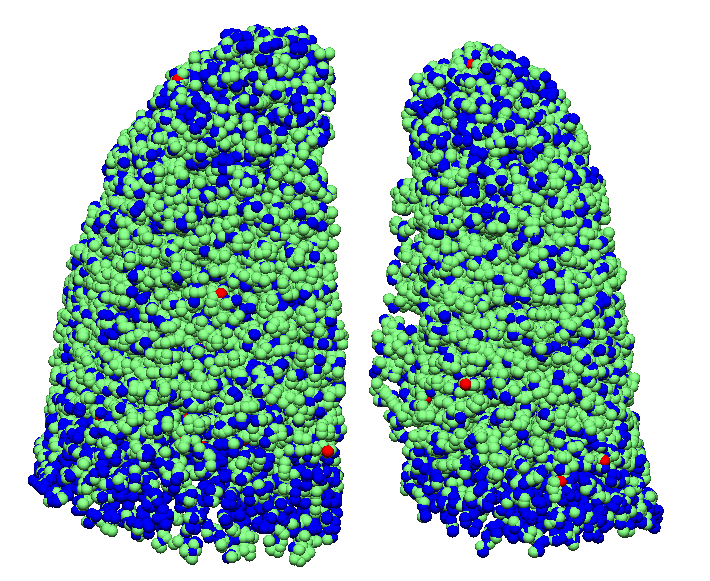
\includegraphics[height=2.9in]{ModelBasedAnalysis/Image/IPF501_DiseaseDistribution_BasedVentilation.png}
  \caption{Disease labeled airway nodes. Green is the normal region, blue is the firbrosis region, and red is the emphysema region.}
  \label{fig:DiseaseLabeling}
\end{figure*}

\subsubsection{Deep inspiration model} 
Deep inspiration model was constructed based on the ventilation model (introduced in Section \ref{ComputationalModelConstruction}) to simulate the deep inspiration from FRC to TLC. For the modeling of old normal people, the reference FRC volume (that is the patient-specific normal volume as reference) from PFT result was used as an initial volume to start inspiration, and the subject-specific muscle pressure was adjusted to drive the lung expand to the target reference TLC volume (acquired from PFT result). For the simulation of IPF patient, the deep inspiration started from the measured FRC volume (acquired from PFT) and the muscle pressure set up in the normal condition was used to guide the lung expansion. Here, we assumed that the inspiratory muscle pressure is normal in IPF patient, as some research indicates that the inspiratory muscle force remains almost the same in IPF lungs compared with normal \citep{de1980inspiratory}. The modeling for IPF patient was divided into two separate stages:

1. The compliance of labeled fibrosis (sum of honeycomb, reticular and ground-glass) acinar unit (connected to its labeled terminal airway node) was reduced to a very low value (less than 0.001 $\mathrm{L/cmH_2O}$) to make sure the fibrosis tissues were stiff enough. Then, inspiration volume was modeled under this fibrosis constricted condition.

2. The deep inspiration volume acquired in Step 1 was used as the target volume, and the tissue compliance of every acinar unit was scaled down together until the simulated inspiration volume can hit the target, then the corresponding scale factor of total tissue compliance was acquired.

\subsubsection{Passive ventilation model}
Time-averaged passive ventilation distribution to each acinus within four breath cycles was predicted using the previously described ventilation model. Acinar volumes were initialized at FRC, using reference normal value and measured disease value, respectively. The scale factor of acinar tissue compliance set in the above Step 2 was applied in the simulation of IPF patient. Patient-specific tidal volume was estimated based on patient's weight, gender and height \citep{gilbert1972changes, pelosi1998effects}.

\subsubsection{Perfusion model}
The perfusion model introduced in Section \ref{ComputationalModelConstruction} was used to estimate the distribution of blood. The individual age, weight, height and gender were integrated to predict the cardiac output for each patient \citep{brandfonbrener1955changes, miyamura1973maximum, stelfox2006hemodynamic}, and the inlet and outlet pressure were adjusted in order to match the estimated cardiac output. The blood vessel radius in fibrosis labeled region was narrowed down for the modeling of IPF, so that the blood flow will be constricted in the lesion area.

\subsubsection{Gas exchange model}
The gas transport and exchange were simulated using the gas exchange model introduced in Section \ref{ComputationalModelConstruction}. The ventilation and perfusion distribution predicted by the ventilation and perfusion model were used as inputs in the normal and disease condition, respectively. Patient-specific oxygen consumption ($\mathrm{VO_2}$) and carbon dioxide consumption ($\mathrm{VCO_2}$) were estimated using the following equations \citep{kwan2004standard, coelho2013estimation}:

\begin{equation} 
 \label{eq:O2ConsumptionEstimation}
 VO_2 = P_{VO_2} \times W,
\end{equation}

\begin{equation} 
 \label{eq:CO2ConsumptionEstimation}
 VCO_2 = VO_2 \times 0.8,
\end{equation}

\noindent where $P_{VO_2}$ is the unit oxygen consumption at rest ($P_{VO_2} = 2.84 \pm 0.34 ml/kg^{-1}/min^{-1}$ for male and $P_{VO_2} = 2.82 \pm 0.37 ml/kg^{-1}/min^{-1}$ for female), and W is the weight of the patient.

With setting up the patient-specific tidal volume and dead space, the partial pressure of oxygen in alveolar ($P_AO_2$) and in arterial blood ($P_aO_2$) can be predicted.
\newpage

%%%%%%%%%%%%%%%%%%%%%%%%%%%%%%%%%%%%%%%%%%%%%%%%%%%%%%%%%%%%%%%%%%%%%%
\section{Results}
\subsection{Construction of lung lobe geometry}
Table \ref{tab:PatientIndividualData} lists the age, BMI and functional measures used for normal lung shape prediction of one patient with IPF. The values were from the patient's individual information, among which FVC, TLC, RV/TLC and DLCO were the patient-specific normal reference values acquired from PFT result. Figure \ref{fig:LungShapePrediction} presents the lung mesh of the IPF patient and its corresponding predicted lung mesh of older normal people. 

\begin{table}[h]
\centering
\caption{Individual information used for normal lung prediction from one patient with IPF}
\label{tab:PatientIndividualData}
\begin{tabular}{| l | c | c| c | c| c | c|}
\hline
\bf{Parameters} & \bf{Age} & \bf{BMI} & \bf{FVC(L)} & \bf{TLC(L)} & \bf{RV/TLC} & \bf{DLCO(mL/mmHg/min)}\\
\hline 
\bf{Values} & 82 & 32.77 & 3.87 & 7.22 & 46 & 25.1\\
\hline
\end{tabular}
\begin{tablenotes}
  \item[1] FVC, TLC, RV/TLC and DLCO are the patient-specific normal reference values acquired from PFT results.
\end{tablenotes}
\end{table}

\begin{figure}[htbp] 
\centering
\begin{subfigure}{.47\linewidth}% set image scale
  \sbox0{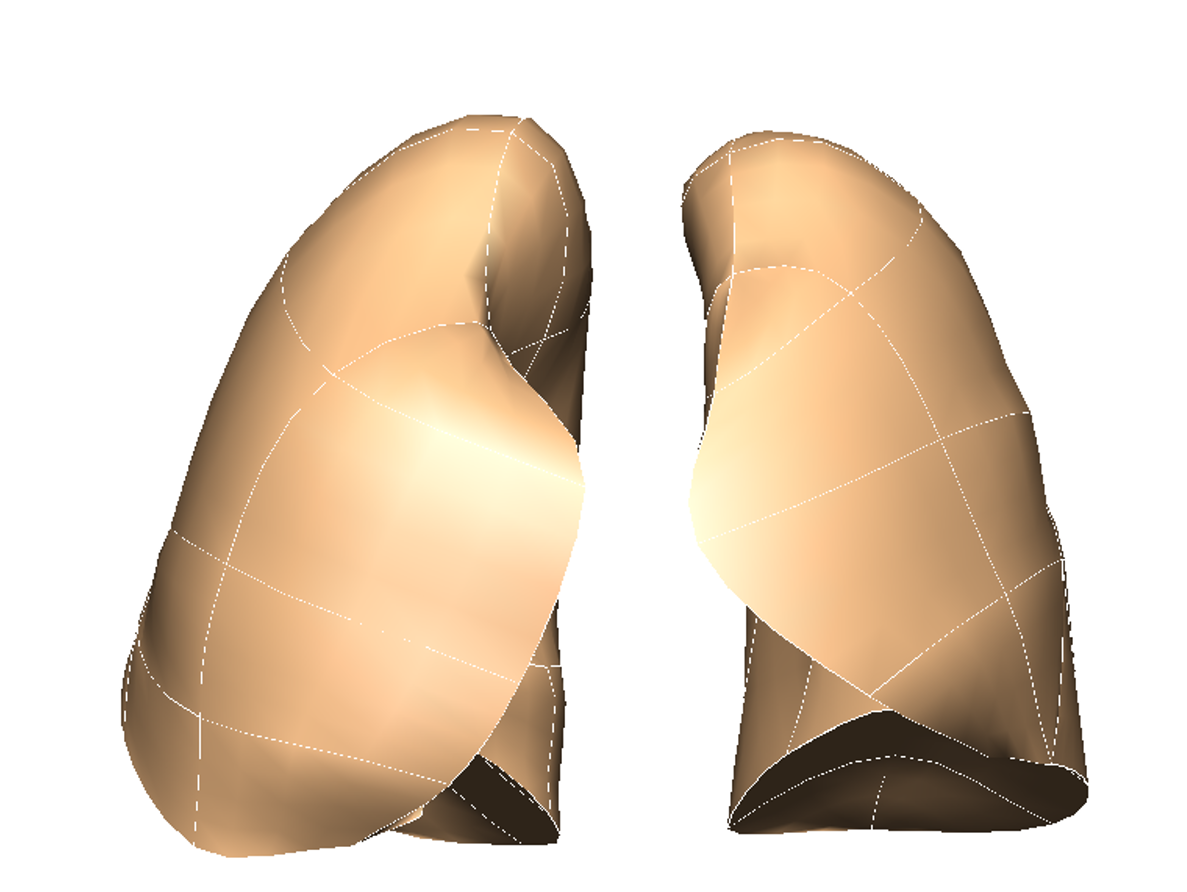
\includegraphics{ModelBasedAnalysis/Image/IPF405_IPFLungMesh.png}}
  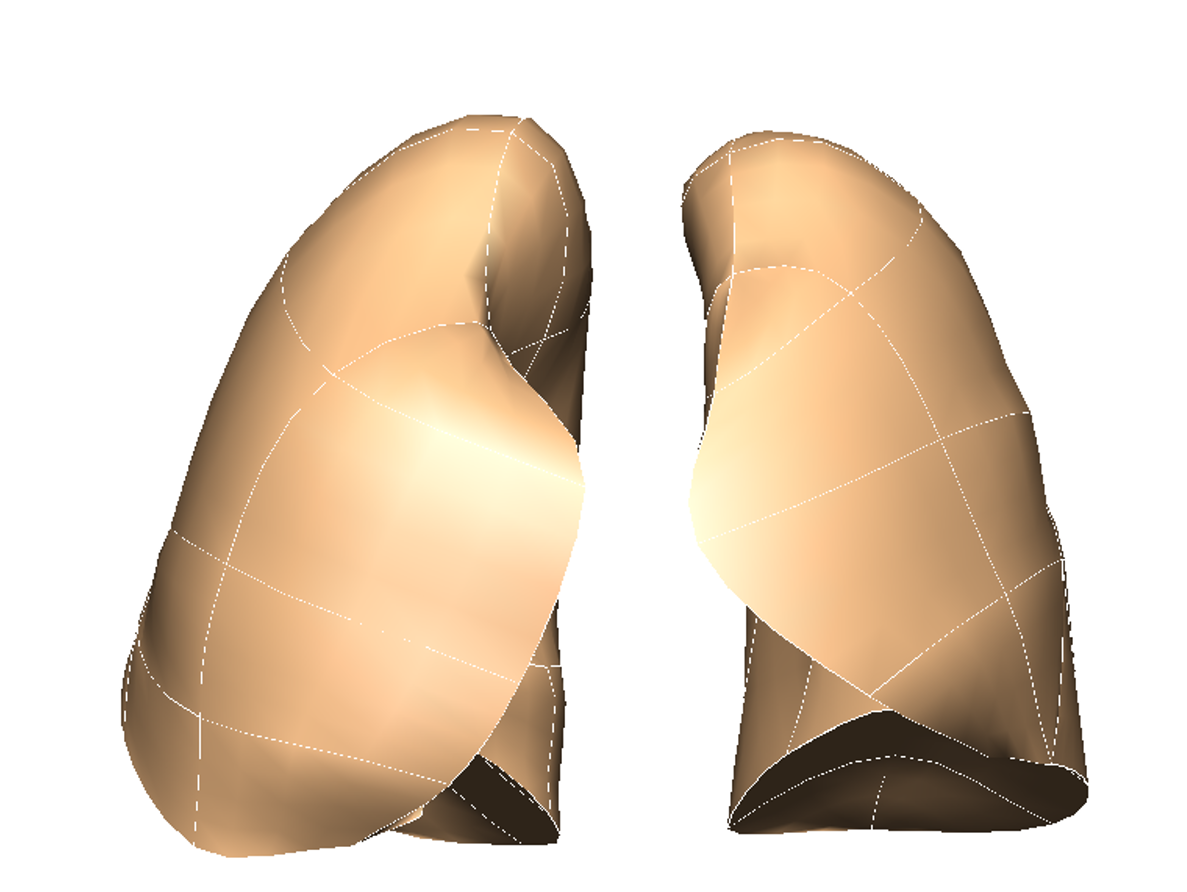
\includegraphics[width=\linewidth,trim={{.0\wd0} {.0\wd0} {.0\wd0} {.0\wd0}},clip]{ModelBasedAnalysis/Image/IPF405_IPFLungMesh.png}
  \caption{IPF lung mesh}
  \label{fig:LungShapePrediction-a} 
\end{subfigure}
%\vspace{.3in} % control space between the upper context and figure
\hspace{.4in} % control space between two figures
\begin{subfigure}{.4\linewidth}% set image scale
  \sbox0{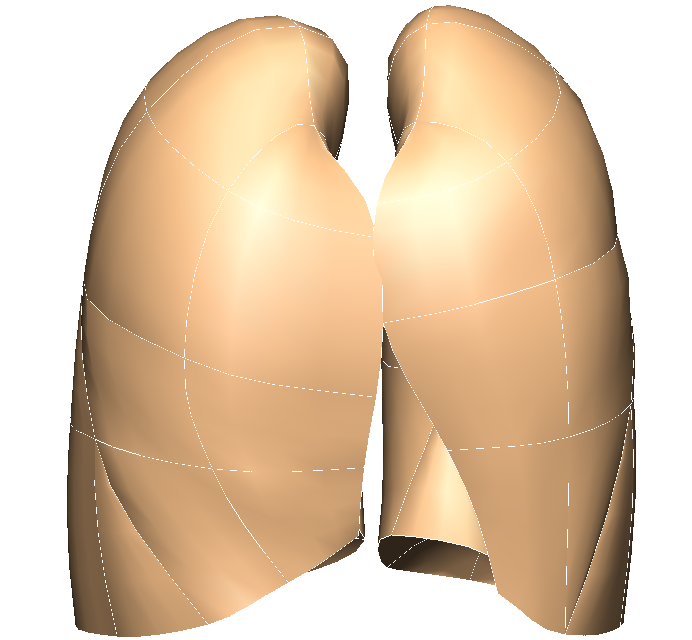
\includegraphics{ModelBasedAnalysis/Image/IPF405_NormalLungMesh.png}}
  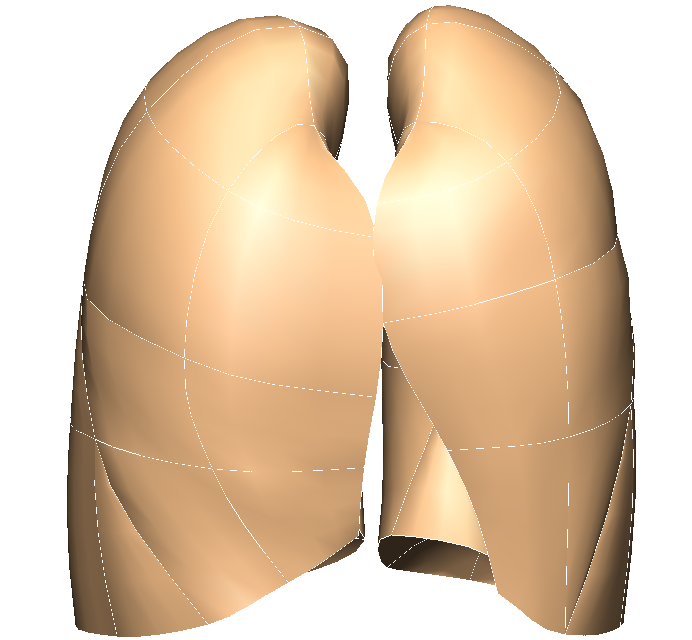
\includegraphics[width=\linewidth,trim={{.0\wd0} {.0\wd0} {.0\wd0} {.0\wd0}},clip]{ModelBasedAnalysis/Image/IPF405_NormalLungMesh.png}
  \caption{Old normal lung mesh}
  \label{fig:LungShapePrediction-b} 
\end{subfigure}
\caption{Lung mesh of IPF and the corresponding predicted lung mesh of old normal. (a) IPF lung mesh generated from CT imaging of a patient with IPF. (b) Old normal lung mesh predicted with the individual information of the same patient.}
\label{fig:LungShapePrediction}
\end{figure}

The average lobe volume proportion of all IPF lung mesh and all predicted old normal lung mesh were calculated, shown in Table \ref{tab:AverageLobeVolume_Predicted}.

%\begin{table}[htbp]
%\centering
%\caption{Average lobe volume proportion of IPF lung mesh and predicted old normal lung mesh.}
%\label{tab:AverageLobeVolume_Predicted}
%\begin{tabular}{| l | c | c |}
%\hline
%\bf{Lobe} & \bf{IPF} & \bf{Predicted old normal} \\
%\hline
%Left lower lobe & 0.2314 & 0.2425\\
%\hline
%Left upper lobe	& 0.2474 & 0.2267\\
%\hline
%Right lower lobe	& 0.2213 & 0.2724\\
%\hline
%Right middle lobe	& 0.1260 & 0.0793\\
%\hline
%Right upper lobe	& 0.1739 & 0.1791\\
%\hline
%\end{tabular}
%\end{table}

\begin{table}[htbp]
\centering
\caption{Average lobe volume proportion of IPF lung mesh and predicted old normal lung mesh.}
\label{tab:AverageLobeVolume_Predicted}
\begin{tabular}{| l | c | c |}
\hline
\bf{Lobe} & \bf{IPF} & \bf{Predicted old normal} \\
\hline
Left lower lobe & 0.231 & 0.242\\
\hline
Left upper lobe	& 0.290 & 0.228\\
\hline
Right lower lobe	& 0.205 & 0.272\\
\hline
Right middle lobe	& 0.130 & 0.078\\
\hline
Right upper lobe	& 0.144 & 0.179\\
\hline
\end{tabular}
\end{table}

As discussed in Chapter 4, Section \ref{SSMBasedAnalysis}, the shape change in IPF lung usually relates to a relatively larger anteroposterior diameter and smaller height of the lung. Meanwhile, IPF lung has a lower average volume proportion for left lower lobe and right lower lobe compared with old normal people. The results illustrated in Figure \ref{fig:LungShapePrediction} and Table \ref{tab:AverageLobeVolume_Predicted} are consistent with our previous findings, with predicted lung mesh of old normal showing a ''thinner'' and ''higher'' shape and lower average volume of left and right lower lobes compared with the IPF mesh generated from CT imaging. 

\subsection{Construction of airway/vasculature geometry}
\subsubsection{Airway tree}
Figure \ref{fig:AirwayGeometry} illustrates the generated airway trees of one IPF patient and its corresponding predicted airway tree of old normal. 

\newgeometry{bottom=2.5cm} %set the left margin of page
\begin{landscape}
\begin{figure}[htbp]
\begin{subfigure}{7.5cm}
    \makebox[60pt]{\raisebox{50pt}{\rotatebox[origin=c]{0}{\minibox{Normal\\ airway}}}}%
    \sbox0{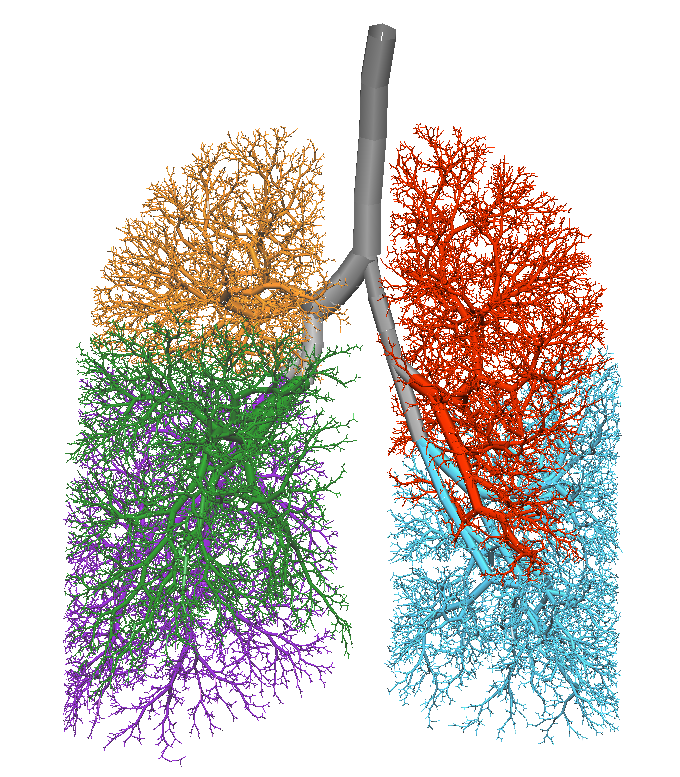
\includegraphics{ModelBasedAnalysis/Image/IPF405_LobeAirway_Normal_1.png}}% get image width, trim={<left> <lower> <right> <upper>}
    \begin{overpic}[height=2.28in,trim={{.0\wd0} {.0\wd0} {.0\wd0} {.0\wd0}},clip]{ModelBasedAnalysis/Image/IPF405_LobeAirway_Normal_1.png}
    \end{overpic}
    \makebox[60pt]{\raisebox{50pt}{\rotatebox[origin=c]{0}{\minibox{IPF\\ airway}}}}% \makebox:change left space, \raisebox: change upper space
    \begin{overpic}[height=2.03in,trim={{.0\wd0} {.0\wd0} {.0\wd0} {.0\wd0}},clip]{ModelBasedAnalysis/Image/IPF405_LobeAirway_Disease_1.png}
    \end{overpic}
    \caption{Anterior view}
		\label{fig:AirwayGeometry-a}
\end{subfigure}\hspace{0.3cm}
\begin{subfigure}{4.9cm}
    \sbox0{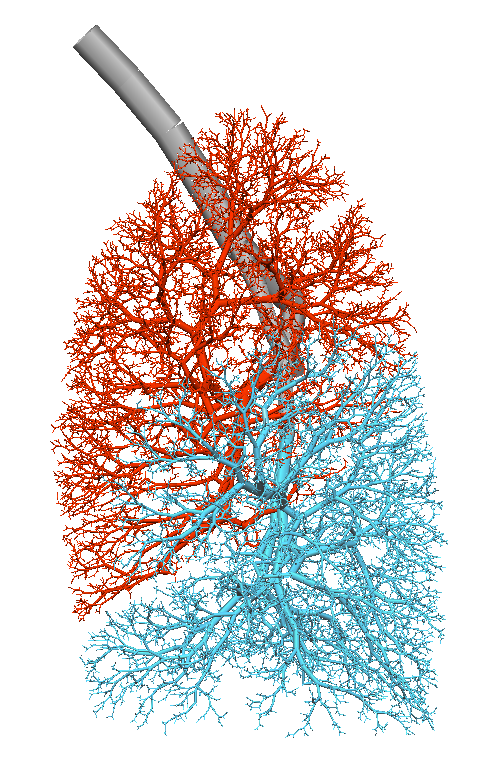
\includegraphics{ModelBasedAnalysis/Image/IPF405_LobeAirway_Normal_2.png}}% get image width, trim={<left> <lower> <right> <upper>}
    \begin{overpic}[height=2.25in,trim={{.0\wd0} {.0\wd0} {.0\wd0} {.0\wd0}},clip]{ModelBasedAnalysis/Image/IPF405_LobeAirway_Normal_2.png}
    \end{overpic}
    \begin{overpic}[height=2.08in,trim={{.0\wd0} {.0\wd0} {.0\wd0} {.0\wd0}},clip]{ModelBasedAnalysis/Image/IPF405_LobeAirway_Disease_2.png}
    \end{overpic}
    \caption{Left lung side}
		\label{fig:AirwayGeometry-b}
\end{subfigure}\hspace{0.3cm}
\begin{subfigure}{4.9cm}
    \sbox0{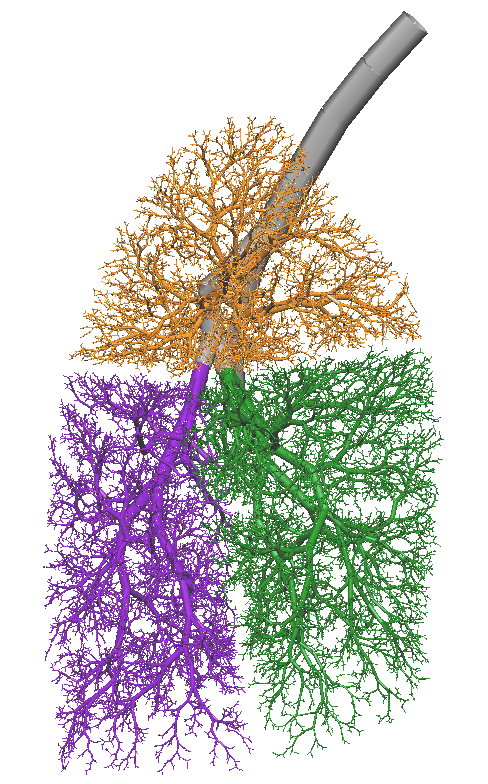
\includegraphics{ModelBasedAnalysis/Image/IPF405_LobeAirway_Normal_3.png}}% get image width, trim={<left> <lower> <right> <upper>}
    \begin{overpic}[height=2.22in,trim={{.0\wd0} {.0\wd0} {.0\wd0} {.0\wd0}},clip]{ModelBasedAnalysis/Image/IPF405_LobeAirway_Normal_3.png}
    \end{overpic}
    \begin{overpic}[height=2.1in,trim={{.0\wd0} {.0\wd0} {.0\wd0} {.0\wd0}},clip]{ModelBasedAnalysis/Image/IPF405_LobeAirway_Disease_3.png}
    \end{overpic}
    \caption{Right lung side}
		\label{fig:AirwayGeometry-c}
\end{subfigure}
\begin{subfigure}{1.7cm}
    \makebox[30pt]{\raisebox{100pt}{\rotatebox[origin=c]{0}{\minibox{\\}}}}
    \sbox0{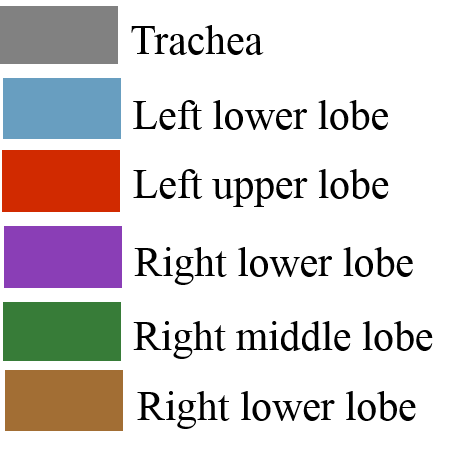
\includegraphics{ModelBasedAnalysis/Image/LobeColors.png}}% get image width, trim={<left> <lower> <right> <upper>}
    \begin{overpic}[height=1.7in,trim={{.0\wd0} {.0\wd0} {.0\wd0} {.0\wd0}},clip]{ModelBasedAnalysis/Image/LobeColors.png}
    \end{overpic}
\end{subfigure}
\caption{Generated normal airway tree (top row) and IPF airway tree (bottom row) for one patient diagnosed with IPF. (a) Anterior view. (b) Left lung side. (c) Right lung side.}
\label{fig:AirwayGeometry}
\end{figure}
\end{landscape}
\restoregeometry

From Figure \ref{fig:AirwayGeometry}, it can be seen that compared with old normal airway tree, IPF airway tree has a larger trachea radius (which is associated with the dilation of conducting airway in IPF lung), a relatively smaller lower lobe and a larger anterioposterior diameter. These features are consistent with the SSM based analysis result of IPF lung shape in Chapter 4, which means our method of generating old normal and IPF airway tree is reasonable and acceptable.

\subsubsection{Vasculature tree}
The generated IPF and old normal vessel trees are shown in Figure \ref{fig:VesselTreeGeometry}. Table \ref{tab:AirwayParameter} lists the parameters used for generating airway tree. Table \ref{tab:VesselParameter} lists the parameters for generating vessel trees. 

\begin{figure}[htbp] 
\centering
\begin{subfigure}{.55\linewidth}% set image scale
  \sbox0{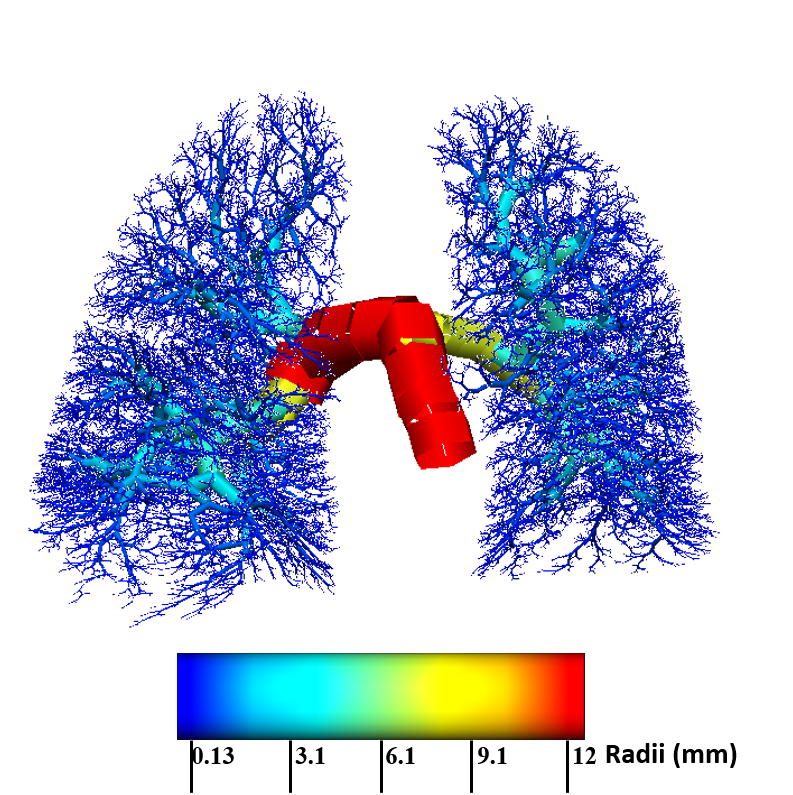
\includegraphics{ModelBasedAnalysis/Image/IPF405_ArteryRadius_IPF.png}}
  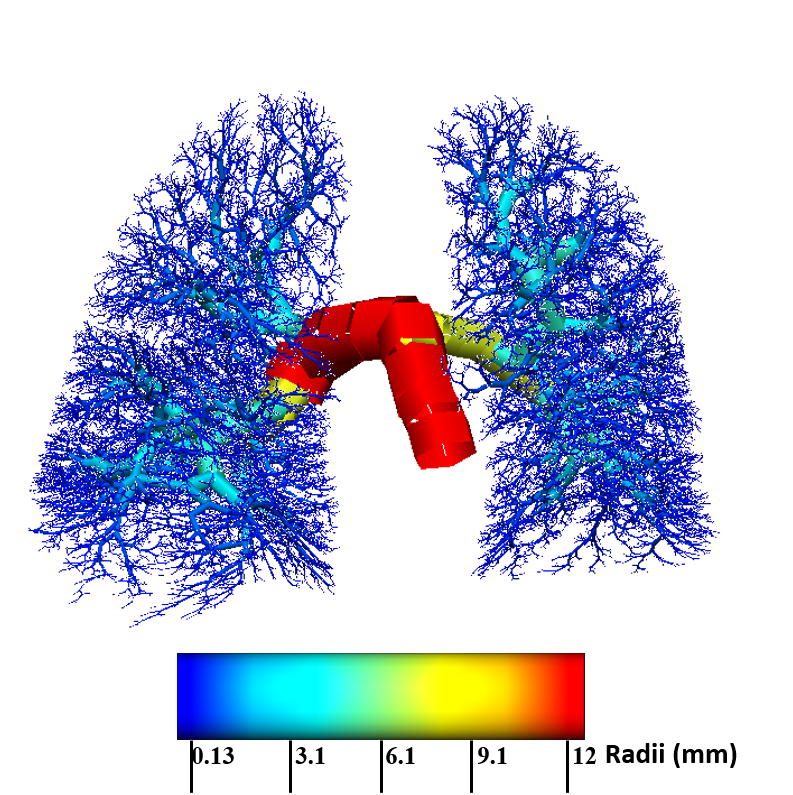
\includegraphics[width=\linewidth,trim={{.0\wd0} {.0\wd0} {.0\wd0} {.0\wd0}},clip]{ModelBasedAnalysis/Image/IPF405_ArteryRadius_IPF.png}
  \caption{IPF vessel tree}
  \label{fig:VesselTreeGeometry-a} 
\end{subfigure}
%\vspace{.1in} % control space between the upper context and figure
\hspace{.1in} % control space between two figures
\begin{subfigure}{.38\linewidth}% set image scale
  \sbox0{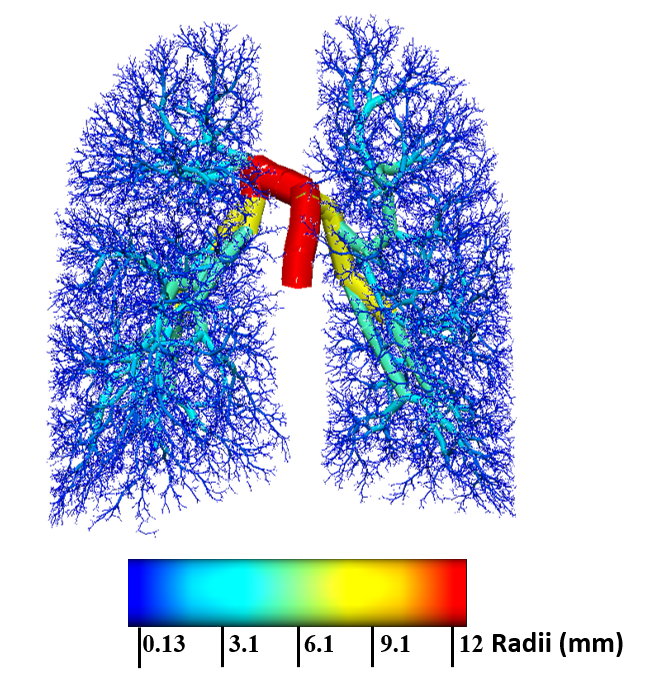
\includegraphics{ModelBasedAnalysis/Image/IPF405_ArteryRadius_Normal.png}}
  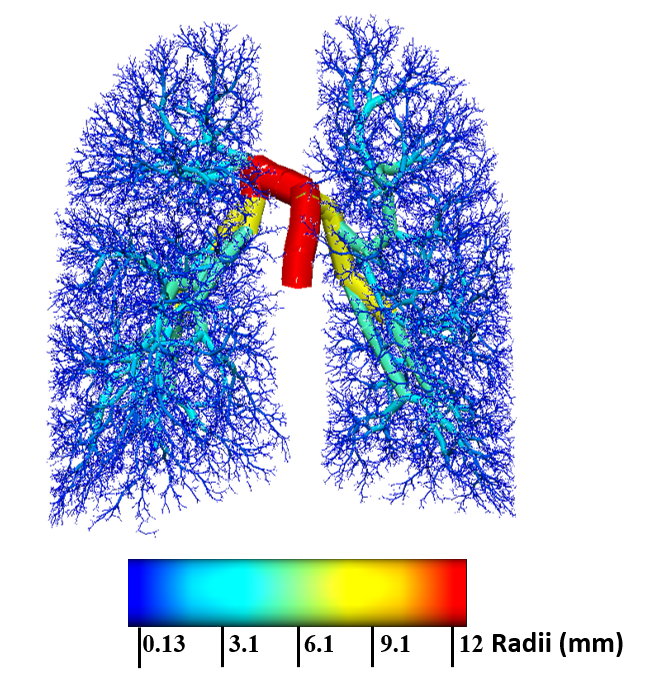
\includegraphics[width=\linewidth,trim={{.0\wd0} {.0\wd0} {.0\wd0} {.0\wd0}},clip]{ModelBasedAnalysis/Image/IPF405_ArteryRadius_Normal.png}
  \caption{Old normal vessel tree}
  \label{fig:VesselTreeGeometry-b} 
\end{subfigure}
\caption{Generated geometry of vessel tree. (a) IPF vessel tree. (b) Old normal vessel tree. The radius of branches were visualized with different colors. The colorbar shows the range of radius.} 
\label{fig:VesselTreeGeometry}
\end{figure}

\newgeometry{bottom=1.0cm} %set the left margin of page
\begin{landscape}
\begin{table}[p]
\centering
\caption{Parameters of old normal and IPF airway tree}
\label{tab:AirwayParameter}
\begin{tabular}{| c | c | c | c | c | c | c | c | c | c |}
\hline
\multirow{2}*{\bf{Patient No.}} & \multirow{2}*{\bf{Time point}} & \multicolumn{2}{|c|}{\bf{Trachea radius (mm)}} & \multicolumn{2}{|c|}{\bf{Horsfield diameter ratio($R_dH$})} & \multicolumn{2}{|c|}{\bf{Terminal radius (mm)}} & \multicolumn{2}{|c|}{\bf{Airway volume (ml)}}\\ 
\cline{3-10}
~ & ~ & Normal & IPF & Normal & IPF  & Normal & IPF & Normal & IPF\\
\hline
\multirow{2}*{Patient 1} & Time point 1 & 6.000 & 8.806 & 1.139 & 1.161  & 0.200 & 0.182 & 76.141 & 99.800\\	
\cline{2-10}
~ & Time point 2 & 6.000 & 9.821 & 1.139 & 1.166  & 0.200 & 0.184 & 75.530 & 123.871\\
\cline{2-10}
~ & Time point 3 & 6.000 & 10.034 & 1.139 & 1.162  & 0.200 & 0.185 & 74.167 & 134.844\\
\hline
\multirow{2}*{Patient 2} & Time point 1 & 6.500 & 9.6778 & 1.137 & 1.159  & 0.200 & 0.180 & 87.701 & 110.993\\	
\cline{2-10}
~ & Time point 2 & 6.500 & 8.708 & 1.137 & 1.154  & 0.200 & 0.182 & 88.851 & 111.150\\
\hline
\end{tabular}
%\begin{tablenotes}
        %\footnotesize
        %\item{IPF511 and IPF501 are two time points from one patient.}
%\end{tablenotes}
\end{table}

\begin{table}[p]
\centering
\caption{Parameters of old normal and IPF vessel tree}
\label{tab:VesselParameter}
\begin{tabular}{| c | c | c | c | c | c | c | c | c | c |}
\hline
\multirow{2}*{\bf{Patient No.}} & \multirow{2}*{\bf{Time point}} & \multicolumn{2}{|c|}{\bf{Main artery radius (mm)}} & \multicolumn{2}{|c|}{\bf{Artery $R_dS$)}} & \multicolumn{2}{|c|}{\bf{Main vein radius (mm)}} & \multicolumn{2}{|c|}{\bf{Vein $R_dS$}}\\ 
\cline{3-10}
~ & ~ & Normal & IPF & Normal & IPF  & Normal & IPF & Normal & IPF\\
\hline
\multirow{2}*{Patient 1} & Time point 1 & 7.69 & 11.28 & 1.45 & 1.51  & 9.17 & 14.66 & 1.48 & 1.54\\	
\cline{2-10}
~ & Time point 2 & 7.69 & 12.58 & 1.45 & 1.52  & 9.17 & 16.75 & 1.48 & 1.56\\
\cline{2-10}
~ & Time point 3 & 7.69 & 12.86 & 1.45 & 1.52  & 9.17 & 17.20 & 1.48 & 1.56\\			
\hline
\multirow{2}*{Patient 2} & Time point 1 & 8.33 & 12.40 & 1.52 & 1.58  & 11.18 & 18.38 & 1.57 & 1.65\\	
\cline{2-10}
~ & Time point 2 & 8.33 & 11.16 & 1.52 & 1.57  & 11.18 & 16.11 & 1.57 & 1.63\\	
\hline
\end{tabular}
%\begin{tablenotes}
        %\footnotesize
        %\item{IPF511 and IPF501 are two time points from one patient.}
%\end{tablenotes}
\end{table}

\end{landscape}
\restoregeometry

\subsection{Deep inspiration modeling}

Table \ref{tab:InspirationVolume} lists the deep inspiration volumes (from FRC to TLC) of reference normal, simulated and measured values (from PFT report). It is shown in the table that the simulated inspiration volume (with CT-based abnormality labeling) of all the time points for these two patients are higher than the measured ones, which means the abnormalities (fibrosis) on the volumetric CT are not sufficient enough to explain the constriction of deep inspiration volume and the increase in lung stiffness of in IPF lung.

\begin{table}[htbp]
\centering
\caption{Reference normal, simulated and PFT measured inspiration volume.}
\label{tab:InspirationVolume}
\begin{tabular}{| c | c | c | c | c |}
\hline
\bf{Patient No.} & \bf{Time point} & \bf{Ref. normal volume} & \bf{Simulated volume} & \bf{Measured volume}\\ 
\hline
\multirow{2}*{Patient 1} & Time point 1 & 1.93 & 1.26 & 1.16\\	
\cline{2-5}
~ & Time point 2 & 1.93 & 1.27 & 1.12 \\
\cline{2-5}
~ & Time point 3 & 1.84 & 1.15 & 1.14\\			
\hline
\multirow{2}*{Patient 2} & Time point 1 & 3.4 & 2.58 & 2.37 \\	
\cline{2-5}
~ & Time point 2 & 3.36 & 2.37 & 1.93 \\	
\hline
\end{tabular}
\end{table}

Based on the inspiration volumes shown in Table \ref{tab:InspirationVolume}, additional fibrosis was added to the CALIPER classified 'normal' tissues until the modeled inspiration volume can match the PFT measured one. Figure \ref{fig:InspirationCurve} shows the inhale pressure curve, CT-based simulated inspiration curve with CAPLIPER fibrosis labeled, and PFT-based simulated inspiration curve with additional fibrosis labeled. With more fibrosis added to the normal region, the inhaled volume is reduced and can match the PFT result. The percentages of CT-based fibrosis (CALIPER classified) and PFT-based fibrosis (CALIPER classified + additional labeled) are listed in Table \ref{tab:FibrosisPercent}.
\newpage 

\begin{figure}[H]
  \centering 
  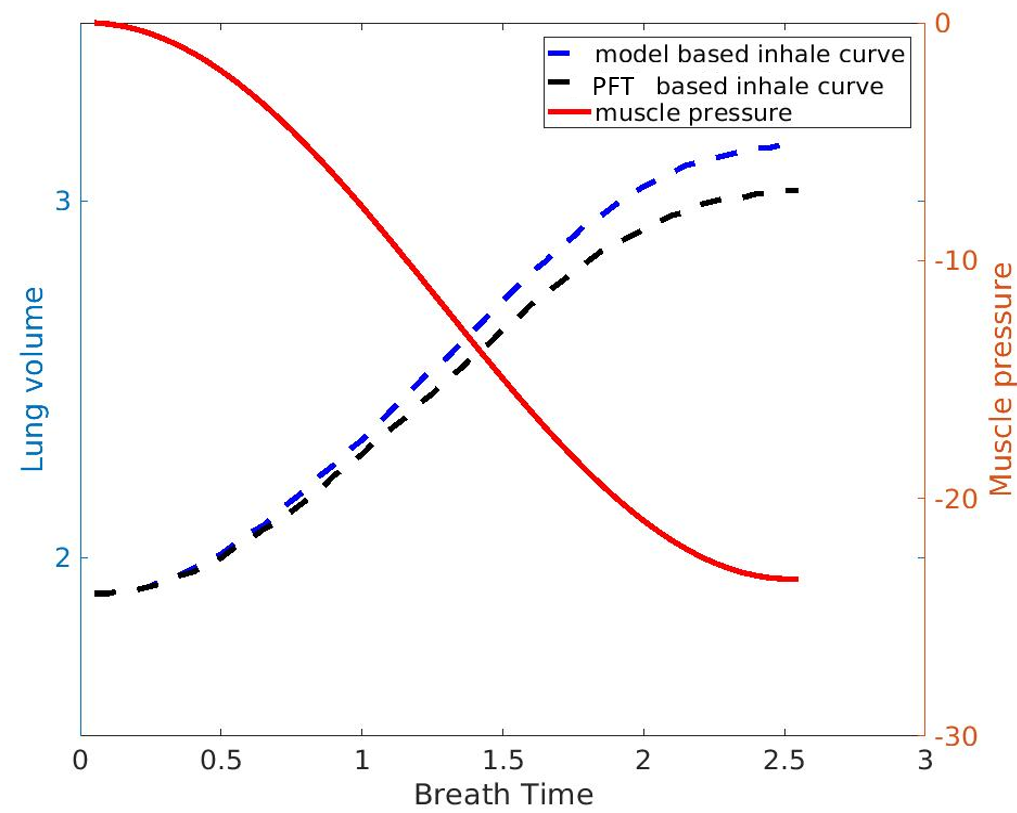
\includegraphics[height=2.9in]{ModelBasedAnalysis/Image/InspirationCurve.png}
  \caption{Deep inspiration and muscle pressure curve. The red line is the muscle pressure curve. The blue lines is the CT-based simulated inspiration curve with CAPLIPER fibrosis labeled, and red line is the PFT-based simulated inspiration curve with additional fibrosis labeled.}
  \label{fig:InspirationCurve}
\end{figure}

\begin{table}[htbp]
\centering
\caption{Percentage of CT-based fibrosis and PFT-based fibrosis.}
\label{tab:FibrosisPercent}
\begin{tabular}{| c | c | c | c |}
\hline
\bf{Patient No.} & \bf{Time point} & \bf{CT-based fibrosis (\%)} & \bf{PFT-based fibrosis (\%)}\\ 
\hline
\multirow{2}*{Patient 1} & Time point 1 & 17.58 & 23.67\\	
\cline{2-4}
~ & Time point 2 & 18.91 & 28.87 \\
\cline{2-4}
~ & Time point 3 & 22.13 & 22.86\\			
\hline
\multirow{2}*{Patient 2} & Time point 1 & 4.26 & 11.86\\	
\cline{2-4}
~ & Time point 2 & 12.46 & 29.12\\	
\hline
\end{tabular}
\end{table}

\subsection{Gas exchange model}
Figure \ref{fig:MIGETFigure} illustrates the distribution of normal, CT-based and PFT-based simulated V/Q ratio and arterial oxygen of one time point from one patient diagnosed with IPF. The figures are shown with V/Q plotted on a logarithmic scale, which is consistent with the presentation of V/Q measurements using the multiple inert gas elimination technique (MIGET). From the results, the simulation for old normal model (the first row) predicts normal V/Q ratio distribution, with $\mathrm{PaO_2}$ of 89.33 mmHg, a typical value of normal older adult. The model labeled with CT-based fibrosispredicts characteristic bimodal V/Q distributions (the second row), and $\mathrm{PaO_2}$ moderately decreased (71.63 mmHg). A slight shift to the left side is observed for the higher peak of V/Q ratio curve compared with the normal model. he small peak of V/Q ratio appears around 5 (larger than 1), as there is a decrease in perfusion in fibrotic area due to the narrowed vessel radius. The model labeled with PFT-based fibrosis predicts appropriate patient-specific FRC and TLC, and decreases in $\mathrm{PaO_2}$ to 67.85 mmHg. The ventilation flow of the higher peak decreases in comparison to the CT-based model, but increases a little bit for the small peak. That is because with more fibrosis labeled on the normal tissue, the lung becomes stiffer. The lower tissue compliance leads to a reduction in total ventilation flow, therefore it can be seen a reduced ventilation of the higher peak. 

\newgeometry{left=2cm} %set the left margin of page
%\begin{landscape}
\begin{figure}[htbp]
\begin{subfigure}{8.5cm}
    \makebox[60pt]{\raisebox{70pt}{\rotatebox[origin=c]{0}{\minibox{\bf{Normal}}}}}%
    \sbox0{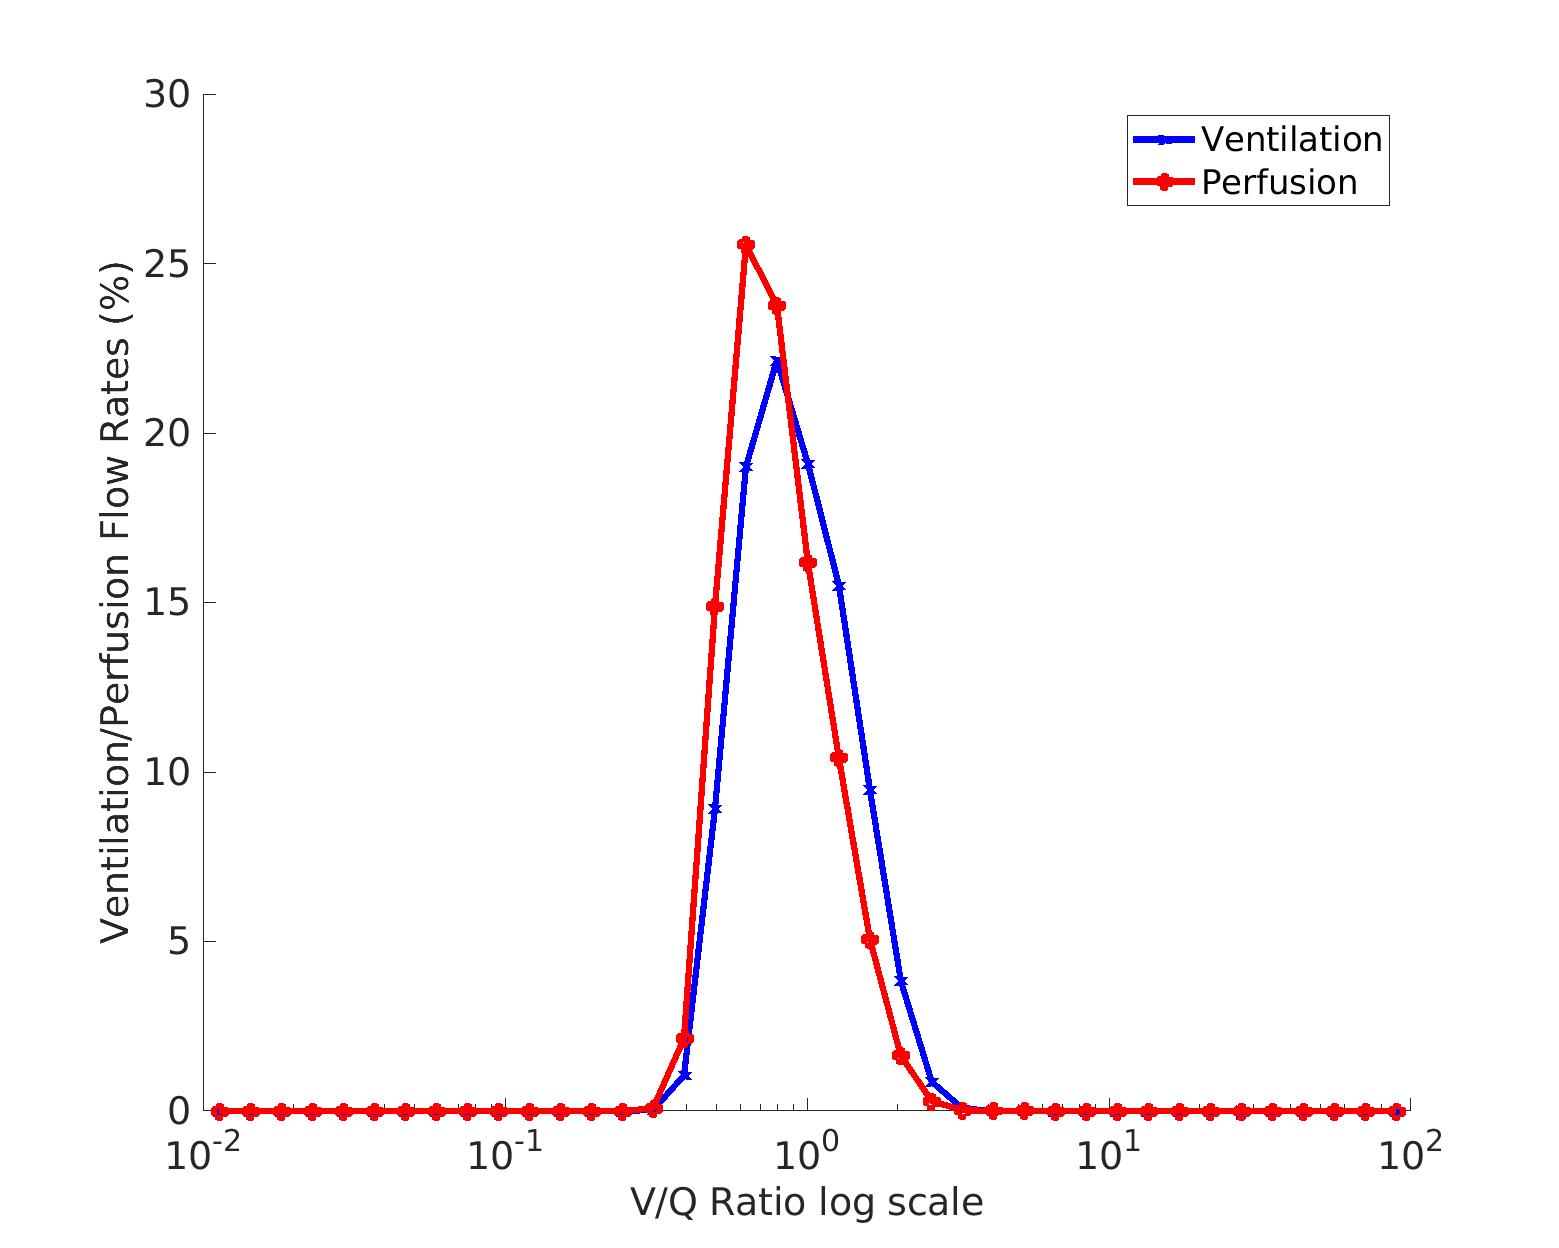
\includegraphics{ModelBasedAnalysis/Image/IPF511_Normal_MIGET_Line_figure.jpg}}% get image width, trim={<left> <lower> <right> <upper>}
    \begin{overpic}[height=2.1in,trim={{.00\wd0} {.00\wd0} {.00\wd0} {.00\wd0}},clip]{ModelBasedAnalysis/Image/IPF511_Normal_MIGET_Line_figure.jpg}
    \end{overpic}
    \makebox[60pt]{\raisebox{70pt}{\rotatebox[origin=c]{0}{\minibox{\bf{CT-based}}}}}% \makebox:change left space, \raisebox: change upper space
    \begin{overpic}[height=2.1in,trim={{.00\wd0} {.00\wd0} {.00\wd0} {.00\wd0}},clip]{ModelBasedAnalysis/Image/IPF511_CTBased_MIGET_Line_figure.jpg}
    \end{overpic}
		\makebox[60pt]{\raisebox{70pt}{\rotatebox[origin=c]{0}{\minibox{\bf{PFT-based}}}}}% \makebox:change left space, \raisebox: change upper space
    \begin{overpic}[height=2.1in,trim={{.00\wd0} {.00\wd0} {.00\wd0} {.00\wd0}},clip]{ModelBasedAnalysis/Image/IPF511_PFTBased_MIGET_Line_figure.jpg}
    \end{overpic}
    \caption{V/Q ratio}
		\label{fig:MIGETFigure-a}
\end{subfigure}\hspace{0.3cm}
\begin{subfigure}{9.0cm}
    \sbox0{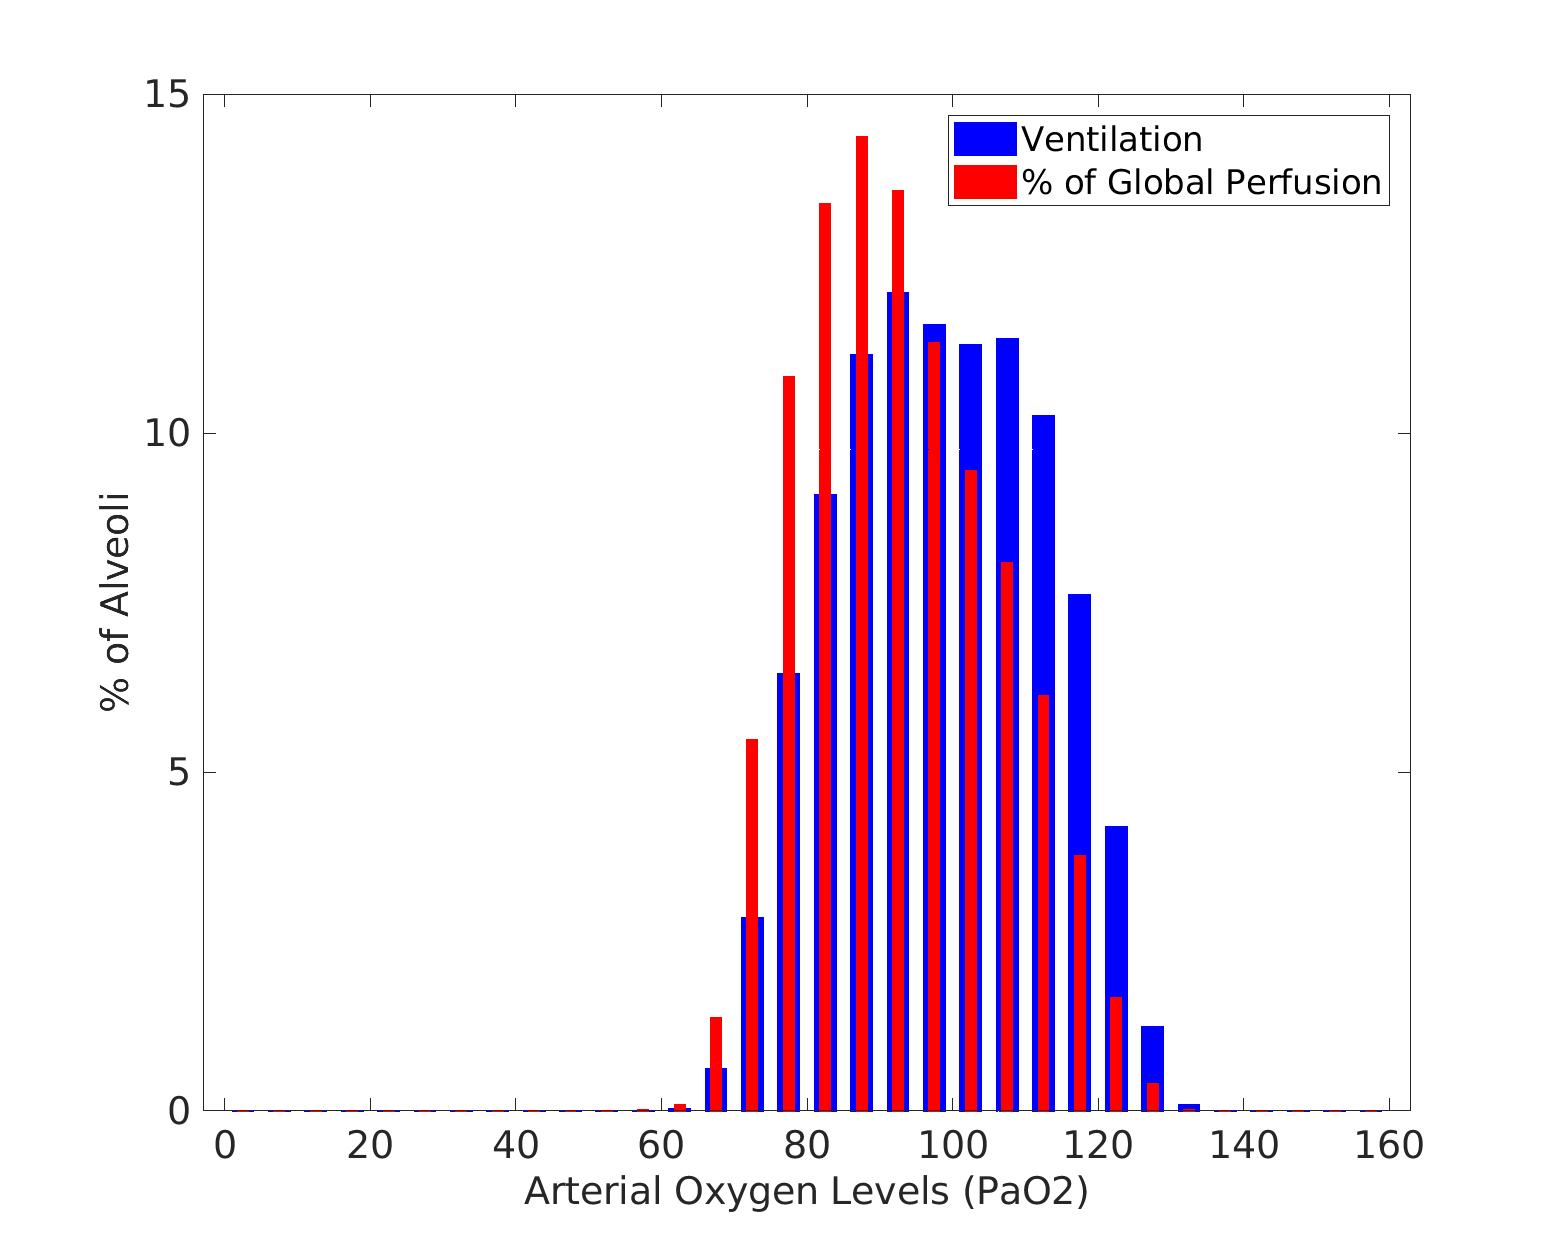
\includegraphics{ModelBasedAnalysis/Image/IPF511_Normal_MIGET_Bar_figure.jpg}}% get image width, trim={<left> <lower> <right> <upper>}
    \begin{overpic}[height=2.1in,trim={{.00\wd0} {.00\wd0} {.00\wd0} {.00\wd0}},clip]{ModelBasedAnalysis/Image/IPF511_Normal_MIGET_Bar_figure.jpg}
    \end{overpic}
    \begin{overpic}[height=2.1in,trim={{.00\wd0} {.00\wd0} {.00\wd0} {.00\wd0}},clip]{ModelBasedAnalysis/Image/IPF511_CTBased_MIGET_Bar_figure.jpg}
    \end{overpic}
    \begin{overpic}[height=2.1in,trim={{.00\wd0} {.00\wd0} {.00\wd0} {.00\wd0}},clip]{ModelBasedAnalysis/Image/IPF511_PFTBased_MIGET_Bar_figure.jpg}
    \end{overpic}
    \caption{Arterial oxygen level}
		\label{fig:MIGETFigure-b}
\end{subfigure}
\caption{V/Q ratio distribution and arterial oxygen distribution of normal, CT-based and PFT-based simulation result of one time point from one patient diagnosed with IPF using MIGET). (a) V and Q flow with respect to V/Q ratio. (b) V and Q percentage with respect to arterial oxygen level.}
\label{fig:MIGETFigure}
\end{figure}
\restoregeometry
%\end{landscape}

Figure \ref{fig:VQDistribution} shows the V, Q and V/Q ratio distribution against lung height (cranio-caudal axis) simulated by older normal, CT-based and PFT-based model. From the result, the ventilation distributes more in lower region than in upper region which is determined entirely by gravity, and there is a left shift for the two IPF simulated ventilation curves compared with the normal one. The mismatch of perfusion between normal model and the two IPF models mainly happens in the basal part of the lung, where more fibrosis appears in these areas. For the old normal simulation, it can be seen an upward trend in V/Q ratio (around 1) with the increasing of lung height, but higher V/Q ratio (V/Q mismatch) is illustrated in CT-based and PFT-based curves, especially in the regions of base and apex.

\begin{figure}[htbp]  
\centering
\begin{subfigure}{.6\linewidth}% set image scale
  \sbox0{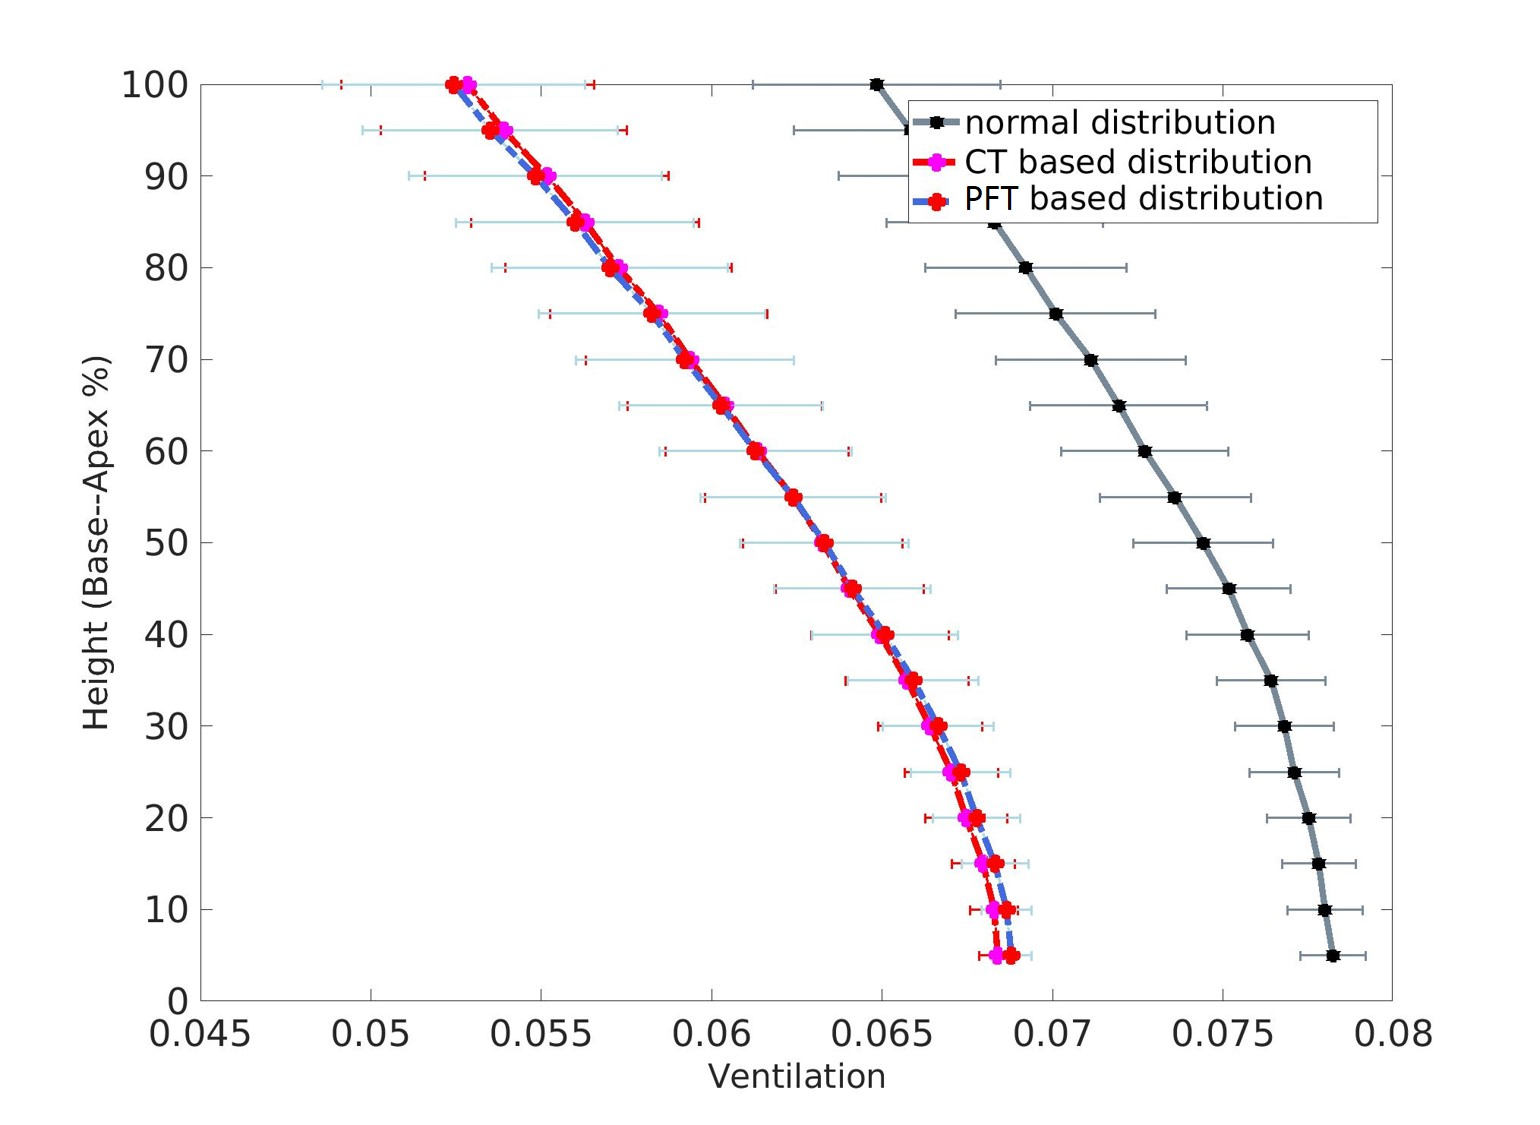
\includegraphics{ModelBasedAnalysis/Image/VentilationAgainstLungHeight.jpg}} 
  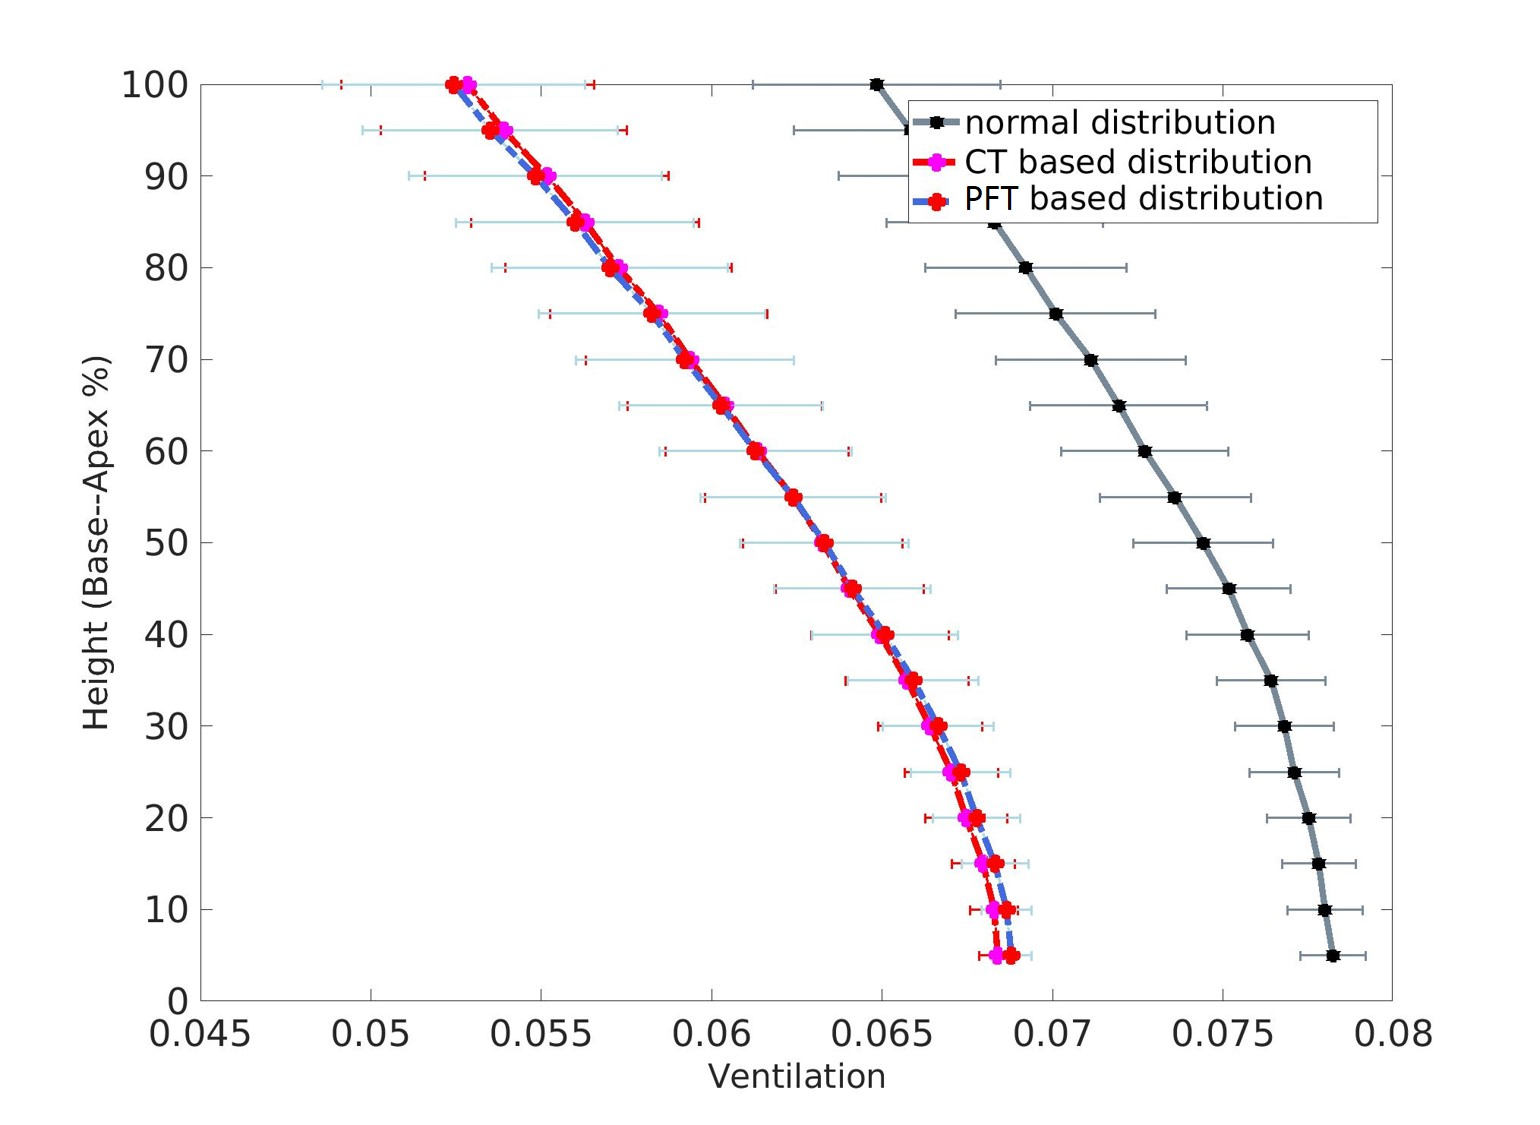
\includegraphics[width=\linewidth,trim={{.0\wd0} {.0\wd0} {.0\wd0} {.0\wd0}},clip]{ModelBasedAnalysis/Image/VentilationAgainstLungHeight.jpg} %trim={<left> <lower> <right> <upper>}, set the cut scale
  \caption{Ventilation distribution}
  \label{fig:VQDistribution-a} 
\end{subfigure} 
\begin{subfigure}{.6\linewidth}% set image scale
  \sbox0{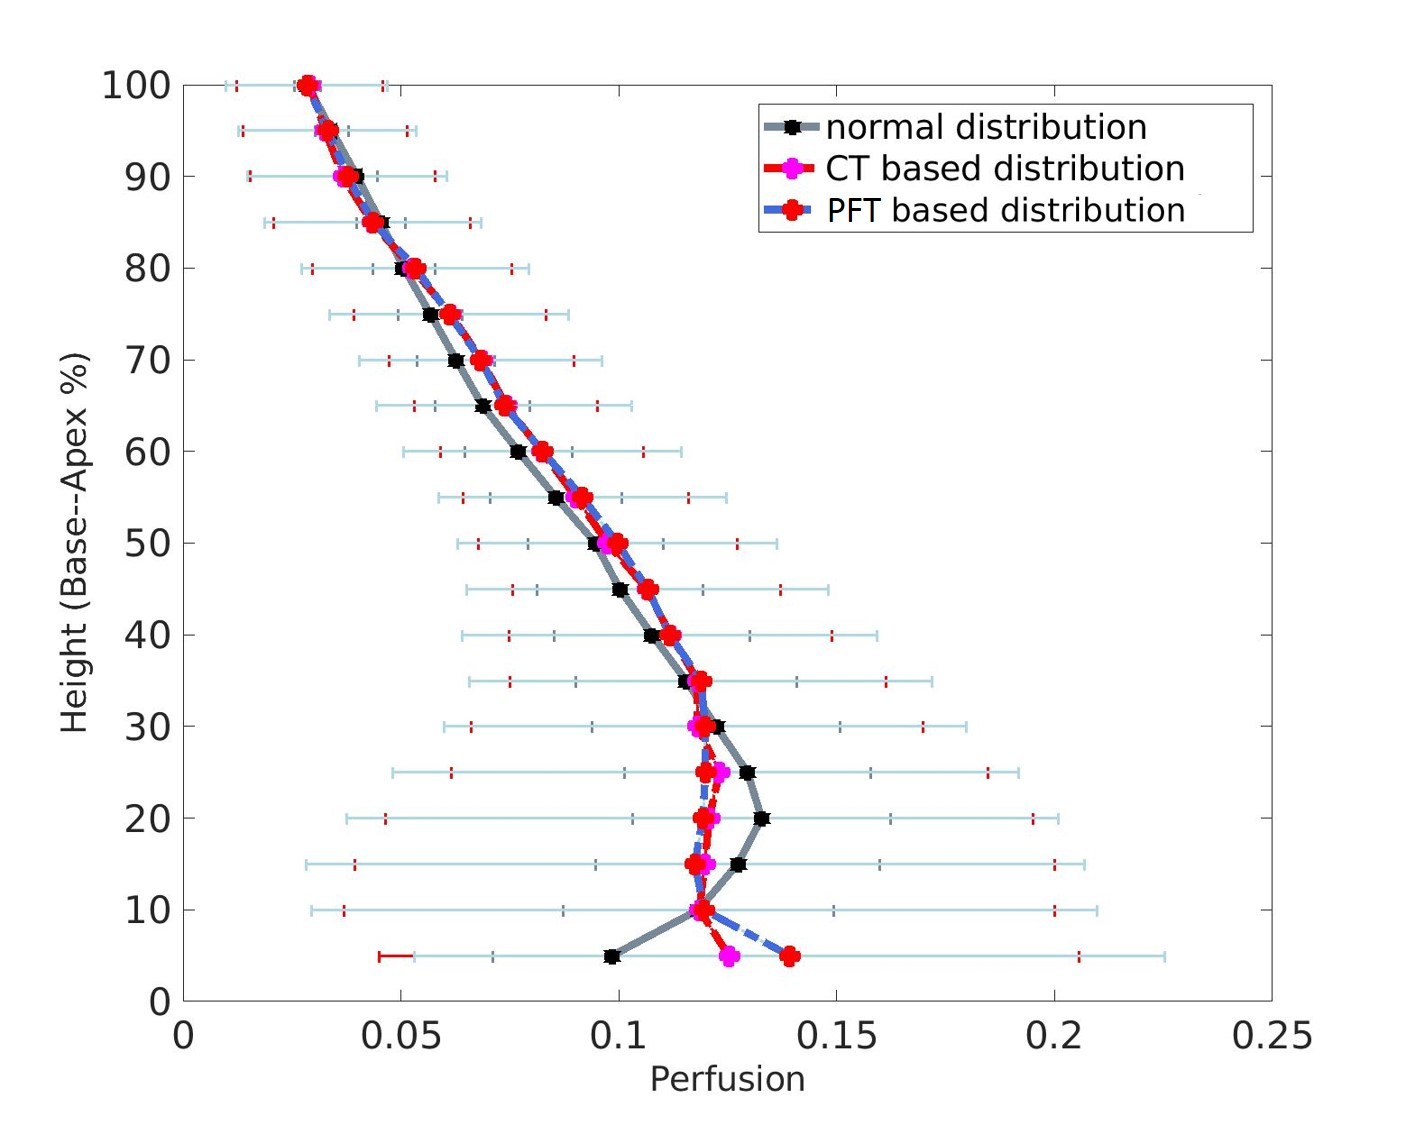
\includegraphics{ModelBasedAnalysis/Image/PerfusionAgainstLungHeight.jpg}}
  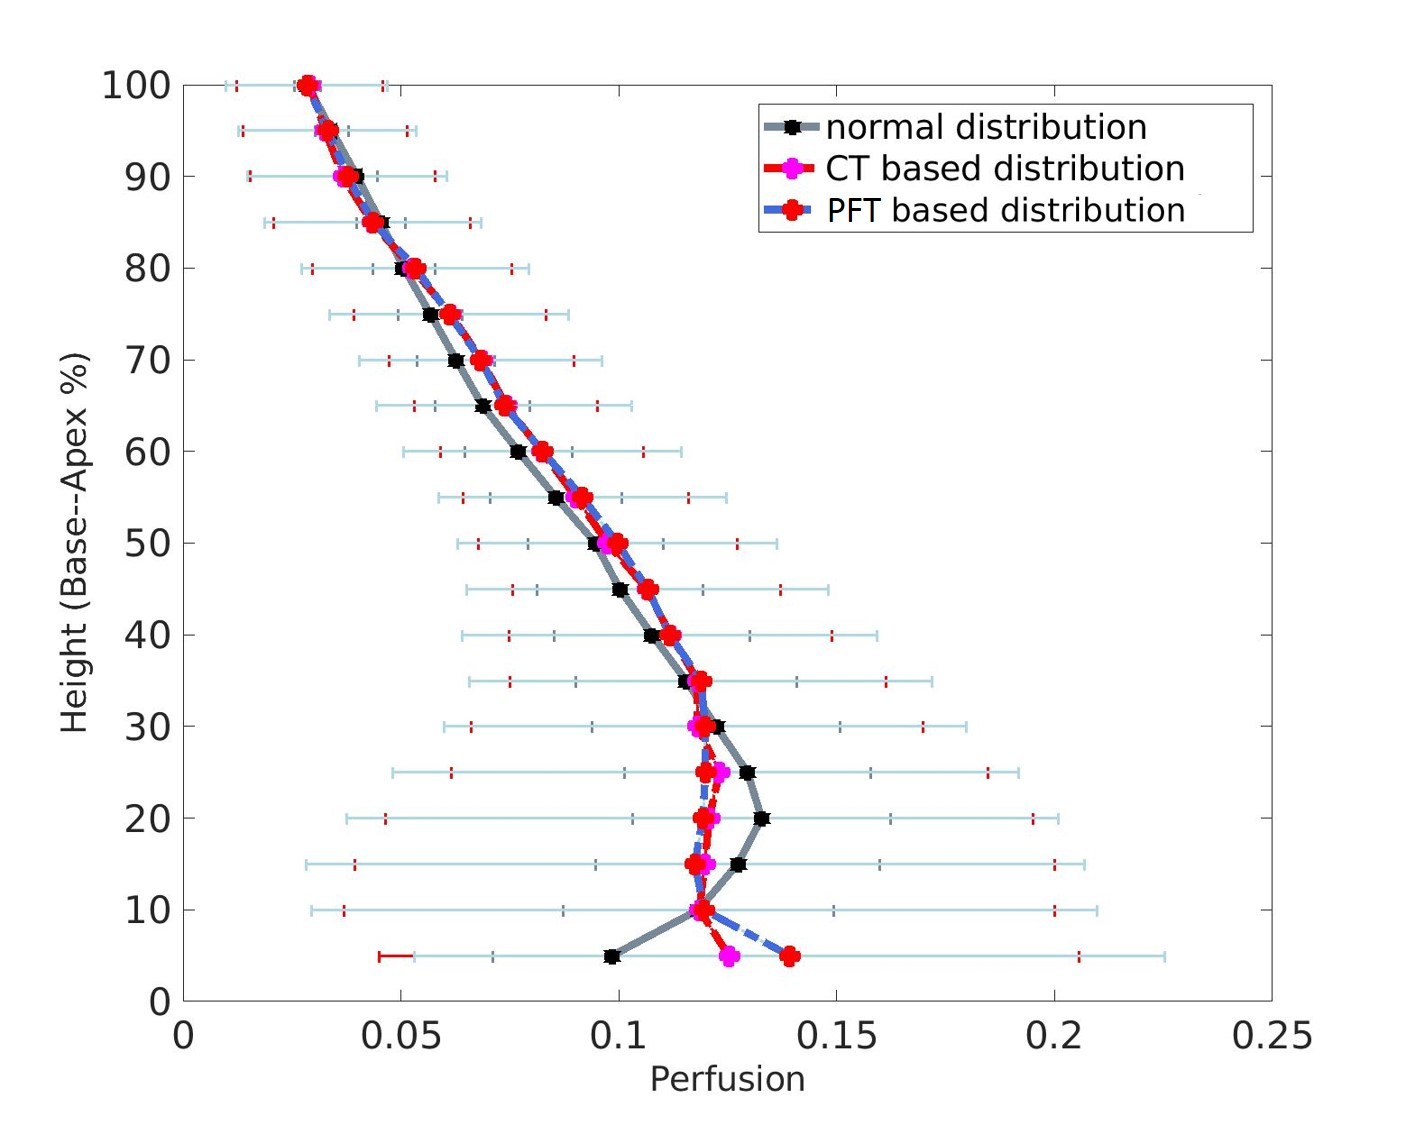
\includegraphics[width=\linewidth,trim={{.0\wd0} {.0\wd0} {.0\wd0} {.0\wd0}},clip]{ModelBasedAnalysis/Image/PerfusionAgainstLungHeight.jpg}
  \caption{Perfusion distribution}
  \label{fig:VQDistribution-b}
\end{subfigure}
\begin{subfigure}{.6\linewidth}% set image scale
  \sbox0{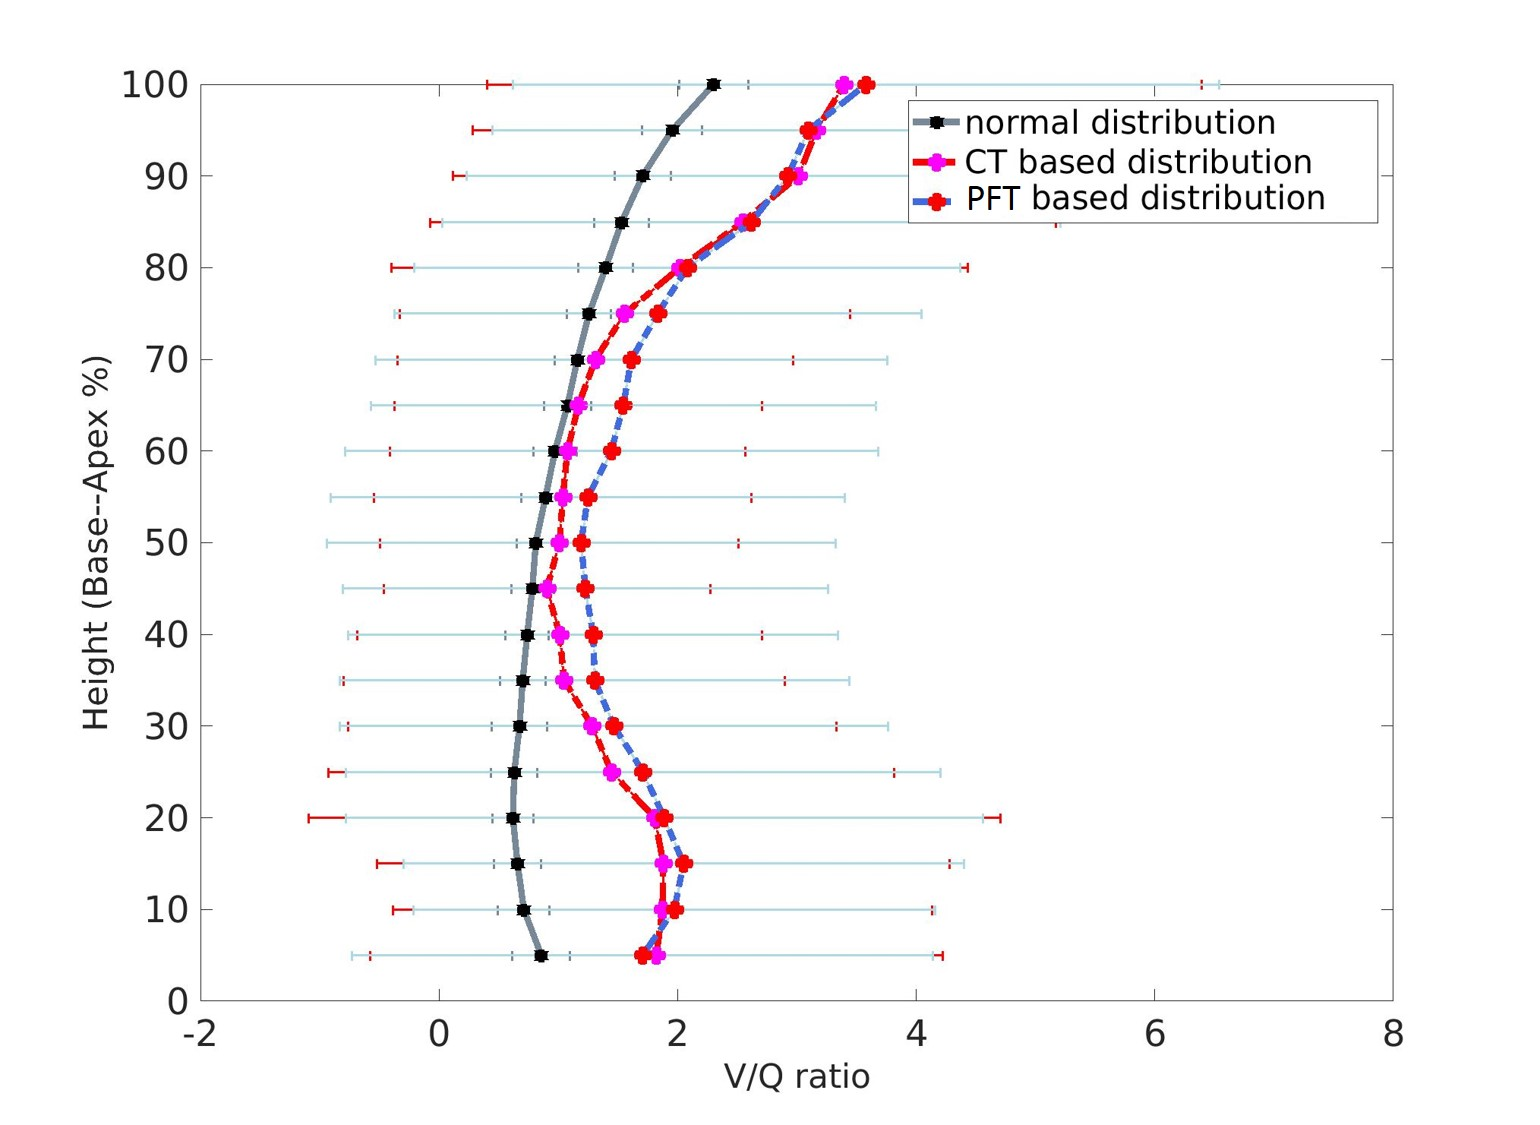
\includegraphics{ModelBasedAnalysis/Image/VQAgainstLungHeight.jpg}}
  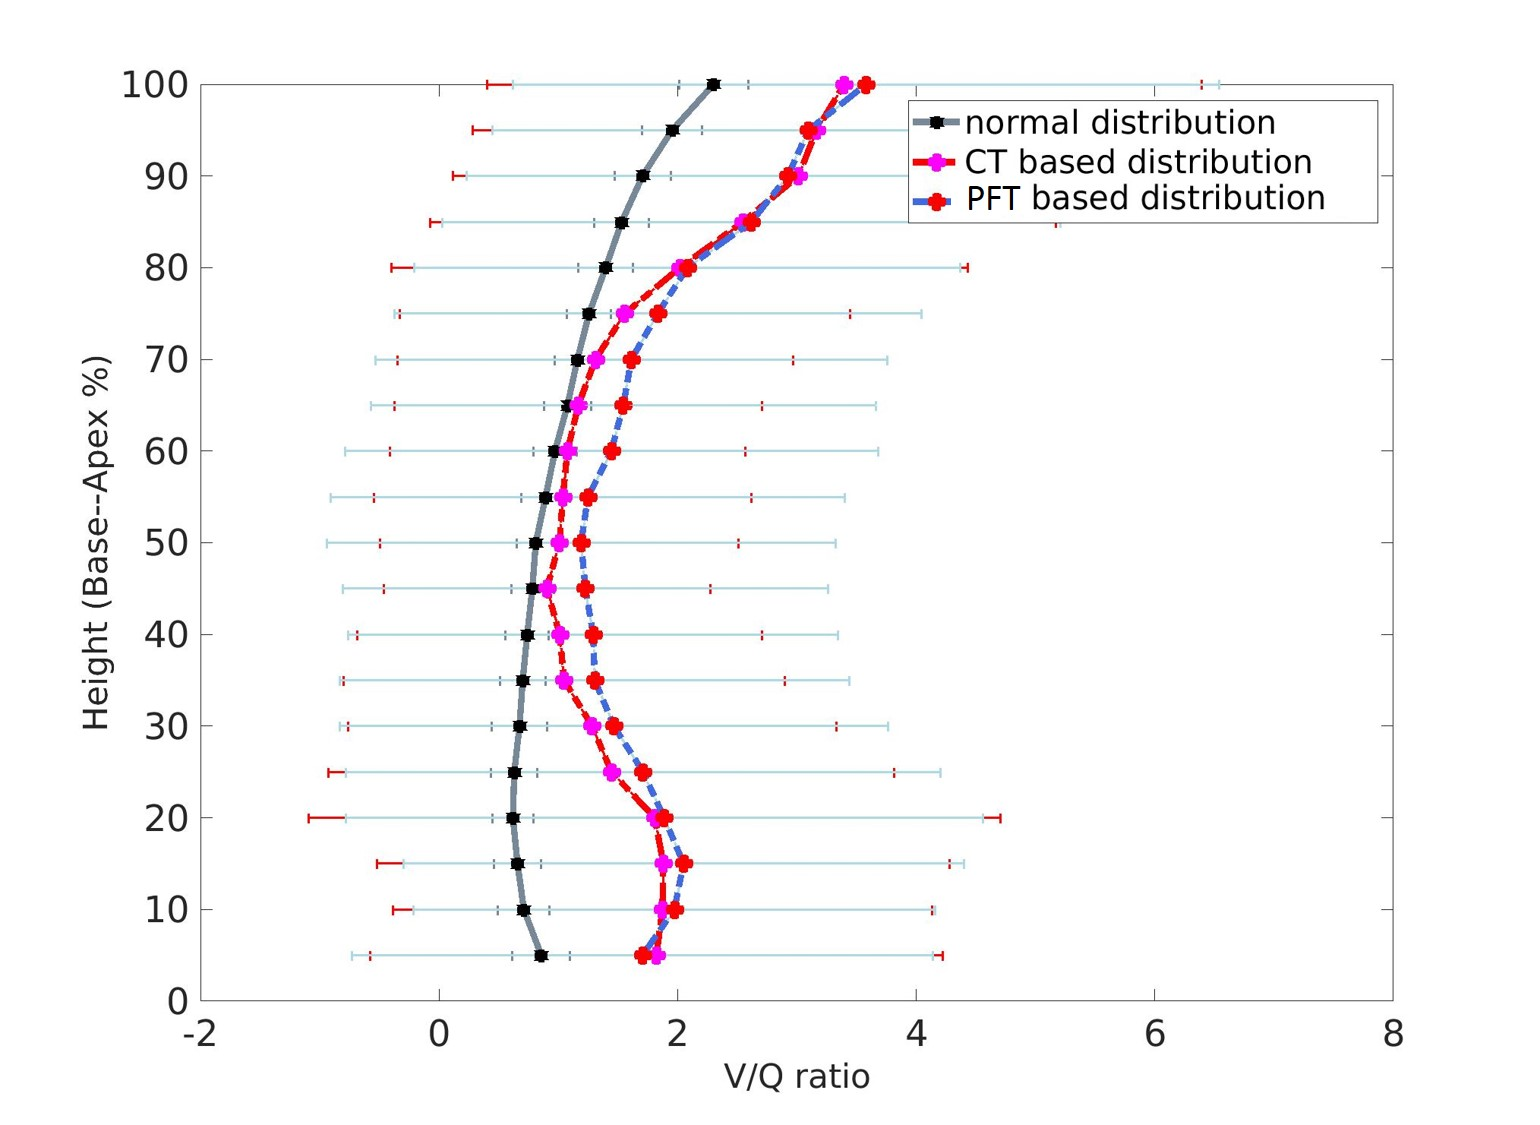
\includegraphics[width=\linewidth,trim={{.0\wd0} {.0\wd0} {.0\wd0} {.0\wd0}},clip]{ModelBasedAnalysis/Image/VQAgainstLungHeight.jpg}
  \caption{V/Q ratio distribution}
  \label{fig:VQDistribution-c}
\end{subfigure}
\caption{ Ventilation, perfusion and V/Q ratio distribution against lung height (cranio-caudal axis). (a) Ventilation distribution against lung height. (b) Perfusion distribution against lung height. (c) V/Q ratio distribution against lung height.}
\label{fig:VQDistribution}
\end{figure}

The values of $\mathrm{PaO_2}$ and $\mathrm{PaCO_2}$ of older normal, CT-based and PFT-based model for each time point of these two patients are listed in Table \ref{tab:PartialPressure}. For CT-based and PFT-based simulation, $\mathrm{PaO_2}$ experiences a decrease over time for both of these two patients, corresponding to the gradual incresement of fibrosis.  MIGET plots of V/Q ratio and arterial oxygen distribution, plots of cranio-caudal distribution of V, Q and V/Q ratio of other subjects and time points can be found in Appendix \ref{appendixMIGET}.

\begin{table}[htbp]
\centering
\caption{Values of $\mathrm{PaO_2}$ and $\mathrm{PaCO_2}$ of older normal, CT-based and PFT-based modeling results.}
\label{tab:PartialPressure}
\begin{tabular}{| c | c | c | c | c | c | c | c |}
\hline
\multirow{2}*{\bf{Patient No.}} & \multirow{2}*{\bf{Time point}} & \multicolumn{3}{|c|}{\bf{$\mathrm{PaO_2}$ (mmHg)}} & \multicolumn{3}{|c|}{\bf{$\mathrm{PaCO_2}$ (mmHg)}}\\ 
\cline{3-8}
~ & ~ & Normal & CT-based & PFT-based & Normal & CT-based & PFT-based\\
\hline
\multirow{2}*{Patient 1} & Time point 1 & 89.33 & 71.63 & 67.85 & 41.87  & 52.73 & 53.97\\	
\cline{2-8}
~ & Time point 2 & 95.37 & 64.56 & 58.72 & 37.81  & 57.48 & 59.58\\
\cline{2-8}
~ & Time point 3 & 87.92 & 60.43 & 60.00 & 42.76  & 59.83 & 59.97\\
\hline
\multirow{2}*{Patient 2} & Time point 1 & 92.31 & 88.52 & 85.13 & 39.80  & 41.74 & 42.86\\	
\cline{2-8}
~ & Time point 2 & 91.72 & 83.70 & 75.35 & 39.09  & 43.77 & 46.76\\
\hline
\end{tabular}
\end{table}

\section{Discussion}
In this chapter, a SSM was used to make a prediction of older normal lung shape for each patient. The SSM based lung shape prediction provides a reliable way to make a comparison of the lung function between a patient-specific lung and its corresponding lung of older normal people. The patient-specific shape prediction was achieved based on the patient's individual information which shows significant correlations with older normal lung shape, therefore the estimated lung shape is able to represent the statistical lung shape of older normal people as a control group. Through modeling the airway/vessel tree and lung function with predicted normal lung mesh, it is possible for us to quantitatively describe the change of respiratory geometry in IPF lung, the decline of lung function, the severity of disease and the prognosis of development. That could be a promising direction for clinical applications in the future.

The computational modeling in this chapter shows that the abnormalities classified by CALIPER from volumetric CT imaging may be not sufficient enough to explain the increase in lung stiffness and the decline of lung function in IPF patient. V/Q mismatch (impaired gas exchange) present in CT-based abnormal tissue as well as regions that are classified as 'normal'. This will truly happen in some patients, due to the low quality of CT scan and the errors caused by mis-classification of tissue patterns. Moreover, for the patients diagnosed at the early of the disease, some 'sub-clinical' symptoms that can not be visualized on radiological imaging can definitely damage to the lung function. So, in a sense, our computational modeling method provides a potential way to work as supplement for the radiological and biopsy diagnosis of IPF, and help the clinicians to make a better decision of treatment planning at a earlier stage. 

However, there are some limitations of the modeling procedure. First, in IPF lung, there is a dilation in trachea, but a constriction in small airway. In this chapter, the trachea radius of normal lung was scaled from the trachea radius of IPF lung using a statistically measured ratio which represents the trachea difference between normal and IPF. The main limitation of this method is the measured ratio may be not accurate enough for all the subjects even though the standard deviation has been taken into consideration in our research. A potential direction in the future work could be to use the change of dead space in IPF lung in the construction of airway geometry. 

Second, the emphysema and the low attenuation area (LAA) are not taken into consideration in this model. Although emphysema classified by CAPLIPER only covers a small proportion of the lung (usually less than 1\%), it is believed to have an impact on the deterioration of lung function together with fibrosis in IPF \citep{cottin2005combined, king2011idiopathic, lin2015combined}. On the other hand, the LAA (mild, moderate and severe) which accounts for a sizable part of the lung may have some correlation with the appearance of emphysema, and both emphysema and LAA are associated with air trapping at the end of inspiration \cite{slebos2015air, hoesein2017air}, which will influence the lung volume at FRC and the change of tissue compliance during breathing. Therefore the emphysema and LAA can to be involved in the future work for setting the initial acinar unit volume at FRC. 

Third, for some end-stage subject with a large proportion fibrotic lesion and a small constricted FRC volume, a larger muscle pressure may be needed to drive the expansion of the stiffer lung, thus the deep inspiration volume probably won't be estimated accurately with a normal muscle pressure. In the future study, the chest wall resting volume can be used to help with setting up the tissue compliance in IPF lung, which is calculated by:

\begin{equation} 
 \label{eq:ChestWallRestingVolume}
 V_{CWRV} = V_{FRC} + C_{cw} \times (-P_{pl}(FRC)),
\end{equation} 

\noindent where $\mathrm{V_{CWRV}}$ is the chest wall resting volume,  $\mathrm{V_{FRC}}$ is the FRC volume, $\mathrm{C_{cw}}$ is the chest wall compliance (fixed to 0.2 $\mathrm{L/cmH_2O}$) and $\mathrm{P_{pl}(FRC)}$ is the pleural pressure at FRC. With a fixed chest wall resting volume for both normal and IPF model, the elastic recoil pressure ($\mathrm{P_e}$) which is determined by pleural pressure will be influenced by the constriction of FRC volume, therefore a correlation can be built between chest wall resting volume and tissue compliance.

%%%%%%%%%%%%%%%%%%%%%%%%%%%%%%%%%%%%%%%%%%%%%%%%
\section{Summary}
In this chapter, a patient-specific computational modeling method was developed to investigate the lung geometry and lung function in IPF patient. In order to make a comparison between IPF patient and older normal people, SSM was used to make a prediction of the lung shape of old normal for each patient, and V/Q distribution and gas exchange were then simulated in normal and IPF condition, respectively, with CALIPER tissue classification data and PFT result as input. The result shows that our computational model can reasonably predict the patient-specific ventilation, perfusion and gas exchange in IPF lung, and quantify the difference of lung function between IPF patient and older normal people. Moreover, it is suggested from the result that the CT imaging may be not able to provide enough information to explain the decline of lung function in IPF patient, and the impaired gas exchange will happen in not only abnormal region but also in CT-visualized 'normal' tissues.
